%% Adaptado a partir de :
%%    abtex2-modelo-trabalho-academico.tex, v-1.9.2 laurocesar
%% para ser um modelo para os trabalhos no IFSP-SPO

\documentclass[
    % -- opções da classe memoir --
    12pt,               % tamanho da fonte
    openright,          % capítulos começam em pág ímpar (insere página vazia caso preciso)
    %twoside,            % para impressão em verso e anverso. Oposto a oneside
    oneside,
    a4paper,            % tamanho do papel. 
    % -- opções da classe abntex2 --
    %chapter=TITLE,     % títulos de capítulos convertidos em letras maiúsculas
    %section=TITLE,     % títulos de seções convertidos em letras maiúsculas
    %subsection=TITLE,  % títulos de subseções convertidos em letras maiúsculas
    %subsubsection=TITLE,% títulos de subsubseções convertidos em letras maiúsculas
    % para pacote url reconhecer hifens como separador
    hyphens,
%    paginasA3,  % indica que vai utilizar paginas em A3 
    % Opções que não devem ser utilizadas na versão final do documento
    draft,              % para compilar mais rápido, remover na versão final
    MODELO,             % indica que é um documento modelo então precisa dos geradores de texto
    TODO,               % indica que deve apresentar lista de pendencias 
    % -- opções do pacote babel --
    english,            % idioma adicional para hifenização
    brazil           % o último idioma é o principal do documento
    ]{ifsp-spo-inf-cpti} % ajustar de acordo com o modelo desejado para o curso

% ---
% Pacotes básicos 
% ---
%\usepackage[utf8]{inputenc}     % Codificacao do documento (conversão automática dos acentos)
% ---

%\usepackage{style}
        


% --- 
% CONFIGURAÇÕES DE PACOTES ADICIONAIS UTEIS
% --- 
\usepackage{pdfpages}			% para incluir arquivos pdf no documento


% ---
% Informações de dados para CAPA e FOLHA DE ROSTO
% ---
\titulo{TÍTULO DO TRABALHO}
\autor{AUTOR DO TRABALHO}

\preambulo{Modelo canônico de trabalho monográfico acadêmico em conformidade com
as normas ABNT apresentado à comunidade de usuários \LaTeX.}

\data{DATA DO TRABALHO}

% Definir o que for necessário e comentar o que não for necessário
% Utilizar o Nome Completo
\orientador{ORIENTADOR}
\coorientador{COORIENTADOR}

% ---


% informações do PDF
\makeatletter
\hypersetup{
        %pagebackref=true,
        pdftitle={\@title}, 
        pdfauthor={\@author},
        pdfsubject={\imprimirpreambulo},
        pdfcreator={LaTeX with abnTeX2 using IFSP model},
        pdfkeywords={abnt}{latex}{abntex}{abntex2}{IFSP}{\ifspprefixo}{trabalho acadêmico}, 
        colorlinks=true,            % false: boxed links; true: colored links
        linkcolor=blue,             % color of internal links
        citecolor=blue,             % color of links to bibliography
        filecolor=magenta,              % color of file links
        urlcolor=blue,
        bookmarksdepth=4
}
\makeatother
% --- 


% ----
% Início do documento
% ----
\begin{document}

% Retira espaço extra obsoleto entre as frases.
\frenchspacing 

%somente para o exemplo, fica primeiro
%\input{00-teste}





% -- lista de pendencias gerada pelo todonotes
% -- altere opções do usepackage para remover na versão final....
\listoftodos
\todo[inline]{remover lista de todo da versão final...}
\newpage

% ----------------------------------------------------------
% ELEMENTOS PRÉ-TEXTUAIS
% ----------------------------------------------------------
\pretextual

% ---
% Capa
% ---
\imprimircapa

\newcounter{todocounter}
\newcommand{\todonum}[2][]
{\stepcounter{todocounter}\todo[#1]{\thetodocounter: #2}}


\todonum[inline]{ajustar titulo do trabalho}
\todonum[inline]{ajustar autor}
\todonum[inline]{ajustar data}
\todonum[inline]{ajustar preambulo}
\todonum[inline]{ajustar curso}
\todonum[inline]{ajustar disciplina}
\todonum[inline]{ajustar departamento}
\todonum[inline]{ajustar orientador/coorientador/professor(es)}
% ---

% ---
% Folha de rosto
% (o * indica que haverá a ficha bibliográfica)
% ---
\imprimirfolhaderosto
%\imprimirfolhaderosto*
% ---

% Quando registrado na biblioteca
%
% ---
% Inserir a ficha bibliografica
% ---

% Isto é um exemplo de Ficha Catalográfica, ou ``Dados internacionais de
% catalogação-na-publicação''. Você pode utilizar este modelo como referência. 
% Porém, provavelmente a biblioteca da sua universidade lhe fornecerá um PDF
% com a ficha catalográfica definitiva após a defesa do trabalho. Quando estiver
% com o documento, salve-o como PDF no diretório do seu projeto e substitua todo
% o conteúdo de implementação deste arquivo pelo comando abaixo:
%
% \begin{fichacatalografica}
%     \includepdf{fig_ficha_catalografica.pdf}
% \end{fichacatalografica}
\begin{fichacatalografica}
    \vspace*{\fill}                 % Posição vertical
    \hrule                          % Linha horizontal
    \begin{center}                  % Minipage Centralizado
    \begin{minipage}[c]{12.5cm}     % Largura
    
    \imprimirautor
    
    \hspace{0.5cm} \imprimirtitulo  / \imprimirautor. --
    \imprimirlocal, \imprimirdata-
    
    \hspace{0.5cm} \pageref{LastPage} p. : il. (algumas color.) ; 30 cm.\\
    
    \hspace{0.5cm} \imprimirorientadorRotulo~\imprimirorientador\\
    
    \hspace{0.5cm}
    \parbox[t]{\textwidth}{\imprimirtipotrabalho~--~\imprimirinstituicao,
    \imprimirdata.}\\
    
    \hspace{0.5cm}
        1. Palavra-chave1.
        2. Palavra-chave2.
        I. Orientador.
        II. Universidade xxx.
        III. Faculdade de xxx.
        IV. Título\\            
    
    \hspace{8.75cm} CDU 02:141:005.7\\
    
    \end{minipage}
    \end{center}
    \hrule
\end{fichacatalografica}
% ---



%Caso necessário
%% ---
% Inserir errata
% ---
\begin{errata}
Elemento opcional da \citeonline[4.2.1.2]{NBR14724:2011}. Exemplo:

\vspace{\onelineskip}


FERRIGNO, C. R. A. \textbf{Tratamento de neoplasias ósseas apendiculares com
reimplantação de enxerto ósseo autólogo autoclavado associado ao plasma
rico em plaquetas}: estudo crítico na cirurgia de preservação de membro em
cães. 2011. 128 f. Tese (Livre-Docência) - Faculdade de Medicina Veterinária e
Zootecnia, Universidade de São Paulo, São Paulo, 2011.

\begin{table}[htb]
\center
\footnotesize
\begin{tabular}{|p{1.4cm}|p{1cm}|p{3cm}|p{3cm}|}
  \hline
   \textbf{Folha} & \textbf{Linha}  & \textbf{Onde se lê}  & \textbf{Leia-se}  \\
    \hline
    1 & 10 & auto-conclavo & autoconclavo\\
   \hline
\end{tabular}
\end{table}

\end{errata}
% ---

%Obrigatório para trabalhos com bancas oficiais
%% ---
% Inserir folha de aprovação
% ---

% Isto é um exemplo de Folha de aprovação, elemento obrigatório da NBR
% 14724/2011 (seção 4.2.1.3). Você pode utilizar este modelo até a aprovação
% do trabalho. Após isso, substitua todo o conteúdo deste arquivo por uma
% imagem da página assinada pela banca com o comando abaixo:
%
% \includepdf{folhadeaprovacao_final.pdf}
%
\begin{folhadeaprovacao}

  \begin{center}
    {\ABNTEXchapterfont\large\imprimirautor}

    \vspace*{\fill}\vspace*{\fill}
    \begin{center}
      \ABNTEXchapterfont\bfseries\Large\imprimirtitulo
    \end{center}
    \vspace*{\fill}
    
    \hspace{.45\textwidth}
    \begin{minipage}{.5\textwidth}
        \imprimirpreambulo
    \end{minipage}%
    \vspace*{\fill}
   \end{center}
        
   Trabalho aprovado. \imprimirlocal, 24 de novembro de 2012:

   \assinatura{\textbf{\imprimirorientador} \\ Orientador} 
   \assinatura{\textbf{Professor} \\ Convidado 1}
   \assinatura{\textbf{Professor} \\ Convidado 2}
   %\assinatura{\textbf{Professor} \\ Convidado 3}
   %\assinatura{\textbf{Professor} \\ Convidado 4}
      
   \begin{center}
    \vspace*{0.5cm}
    {\large\imprimirlocal}
    \par
    {\large\imprimirdata}
    \vspace*{1cm}
  \end{center}
  
\end{folhadeaprovacao}
% ---


% ---- opcionais 
% ---
% Dedicatória
% ---
\begin{dedicatoria}
   \vspace*{\fill}
   \centering
   \noindent
   \textit{ Este trabalho é dedicado ao público neurodiverso que\\
   merece, assim como todos, respeito.} 

%\todonum[inline]{colocar sua dedicatoria}
   
   \vspace*{\fill}
   

\end{dedicatoria}
% ---
% ---
% Agradecimentos
% ---
\begin{agradecimentos}
%\todonum[inline]{colocar seus agradecimentos}
Os agradecimentos principais são direcionados à Gerald Weber, Miguel Frasson,
Leslie H. Watter, Bruno Parente Lima, Flávio de Vasconcellos Corrêa, Otavio Real
Salvador, Renato Machnievscz\footnote{Os nomes dos integrantes do primeiro
projeto abn\TeX\ foram extraídos de
\url{http://codigolivre.org.br/projects/abntex/}} e todos aqueles que
contribuíram para que a produção de trabalhos acadêmicos conforme
as normas ABNT com \LaTeX\ fosse possível.

Agradecimentos especiais são direcionados ao Centro de Pesquisa em Arquitetura
da Informação\footnote{\url{http://www.cpai.unb.br/}} da Universidade de
Brasília (CPAI), ao grupo de usuários
\emph{latex-br}\footnote{\url{https://groups.google.com/group/latex-br}} e aos
novos voluntários do grupo
\emph{\abnTeX}\footnote{\url{https://groups.google.com/group/abntex2} e
\url{http://abntex2.googlecode.com/}}~que contribuíram e que ainda
contribuirão para a evolução do \abnTeX.

\end{agradecimentos}
% ---
% ---
% Epígrafe
% ---
\begin{epigrafe}
    \vspace*{\fill}
    \begin{flushright}
        \textit{``Não vos amoldeis às estruturas deste mundo, \\
        mas transformai-vos pela renovação da mente, \\
        a fim de distinguir qual é a vontade de Deus: \\
        o que é bom, o que Lhe é agradável, o que é perfeito.''\\
        (Bíblia Sagrada, Romanos 12, 2)}
    \end{flushright}
\end{epigrafe}
% ---

% -- resumo obrigatório
% ---
% RESUMOS
% ---

% resumo em português
\setlength{\absparsep}{18pt} % ajusta o espaçamento dos parágrafos do resumo
\begin{resumo}

Com o crescimento exponencial do uso da internet na última década, as redes sociais se mostraram o maior centro de socialização da sociedade moderna, local em que são pautadas uma infinidade de assuntos. Percebendo que, em meio a essa infinidade, existe a necessidade de evidenciação de algumas dessas pautas por vezes negligenciadas frente aos tópicos dominantes nas redes, surge o diversaGente. Esse é um aplicativo de rede social focado na melhoria de vida de pessoas com neurodiversidades e suas famílias a partir da criação de um ambiente em que elas sintam-se confortáveis para trocar experiências. E para tornar esse app possível, a metodologia ágil seguida para organizar e desenvolver do projeto baseia-se Scrum. Além disso, toda a documentação foi construída de acordo com as regras \ac{ABNT} e as tecnologias utilizadas no desenvolvimento integram o ecossistema JavaScript, as quais incluem React Native, Typescript, Node.JS, Nest.JS e Prisma.

 \textbf{Palavras-chaves}: rede social. neurodiversidades. projeto.

\end{resumo}

% resumo em inglês
\begin{resumo}[Abstract]
 \begin{otherlanguage*}{english}

With the exponential growth of internet usage in the last decade, social networks proved to be the biggest center of socialization of modern society, where it can be find a multitude of subjects. Realizing that in the midst of this infinity there is a necessity of highlighting some of these themes that are sometimes neglected in comparison to the mainstream topics on the social media, the diversaGente appears. It is a social network app focused on improving the lives of people with neurodiversities and their family by creating an environment where they feel comfortable to exchange experiences. And to build this app, the agile methodology followed to organize and develop the project is based on Scrum. In addition, the complete documentation complies with the \ac{ABNT} rules and the technologies used in development are part of the JavaScript ecosystem, which includes React Native, Typescript, Node.JS, Nest.JS and Prisma.

   \textbf{Keywords}: social networks. neurodiversities. project.
 \end{otherlanguage*}
\end{resumo}


% ---
% inserir lista de ilustrações
% ---
\pdfbookmark[0]{\listfigurename}{lof}
\listoffigures*
\cleardoublepage
% ---

% ---
% inserir lista de tabelas
% ---
\pdfbookmark[0]{\listtablename}{lot}
\listoftables*
\cleardoublepage
% ---

% ---
% inserir lista de quadros
% ---
\pdfbookmark[0]{\listofquadrosname}{loq}
\listofquadros*
\cleardoublepage
% ---

% ---
% inserir lista de abreviaturas e siglas
% ATENCAO o SHARELATEX GERA O GLOSSARIO SOMENTE UMA VEZ
% CASO SEJA FEITA ALGUMA ALTERAÇÃO NA LISTA DE SIGLAS É NECESSARIO UTILIZAR A OPÇÃO :
% "Clear Cached Files" DISPONIVEL NA VISUALIZAÇÃO DOS LOGS 
% ---
% https://www.sharelatex.com/learn/Glossaries


\ifdef{\printnoidxglossary}{
    \printnoidxglossary[type=\acronymtype,title=Lista de abreviaturas e siglas,style=siglas]
    \cleardoublepage
ssh}{}


% ---
% inserir lista de símbolos
% ---
\begin{simbolos}
  \item[$ \Gamma $] Letra grega Gama
  \item[$ \Lambda $] Lambda
  \item[$ \zeta $] Letra grega minúscula zeta
  \item[$ \in $] Pertence
\end{simbolos}
% ---

\todo[inline]{Remover lista de simbolos se não for necessário}


% ---
% inserir o sumario
% ---
\pdfbookmark[0]{\contentsname}{toc}
\tableofcontents*
\cleardoublepage
% ---


% ----------------------------------------------------------
% ELEMENTOS TEXTUAIS
% ----------------------------------------------------------
\textual


% ----------------------------------------------------------
% Introdução
% ----------------------------------------------------------
\chapter[Introdução]{Introdução}

Dispositivos móveis são amplamente utilizados pelos brasileiros, em 2019 82,7\% dos domicílios brasileiros possuíam acesso à Internet, e 98,6\% deles o faziam através de um telefone celular \cite{ibge2019}. Com este alto índice de uso surge também a grande popularidade das redes sociais no país e, por consequência da facilidade de disseminar informação, a necessidade de encontrar lugares confiáveis para se compartilhar e receber informações.

As redes sociais possibilitam a interação de milhões de pessoas, integrando grupos variados de diferentes lugares em um único ambiente virtual. Essas redes funcionam muito bem para lidar com as necessidades de interação da maioria das pessoas, mas não é possível afirmar que se encaixam perfeitamente para todos, afinal, existem públicos que requerem atenção diferenciada, um exemplo deles são as pessoas neurodiversas, que vivenciam uma rotina completamente destoante do convencional.

As barreiras e preconceitos que pessoas neurodiversas enfrentam na sociedade se iniciam já na dificuldade de acesso à informações corretas e confiáveis sobre o próprio termo que as englobam: neurodiversidade. Um termo designado à condição de pessoas cuja neurobiologia se desenvolveu de forma atípica em relação a um parâmetro médico e biológico que se designa como desenvolvimento normal na espécie humana. O T\ac{tdah} e o \ac{tea} são exemplos de diagnósticos comuns às pessoas neurodiversas e, apesar de todo o avanço científico dos últimos anos que possibilitam cada vez maior qualidade de vida, existem muitas barreiras de âmbito social que estas pessoas ainda enfrentam. Diante desse cenário, a socialização de milhares de pessoas neurodiversas é prejudicada e, muitas vezes, descredibilizada, e dado que o ser humano é um ser inerentemente social, o que ocorre é que elas têm uma necessidade elementar debilitada e por inúmeras vezes ignorada \cite{kanner43}.

Todo responsável por uma criança neurodiversa compreende a dificuldade existente desde o momento do diagnóstico, momento que traz uma enorme insegurança sobre como se dará o futuro da criança, até questões vistas como básicas do dia a dia. Atualmente, pouco se fala sobre as neurodiversidades, mas com pouca pesquisa pode-se descobrir que várias das pessoas que apresentam essas condições podem ter uma vida dita socialmente como normal, conseguindo brincar, estudar, trabalhar e construir relacionamentos sólidos, assim como outra pessoa não neurodiversa. O ponto de diferença é que, aquele que é diagnosticado com alguma divergência neurológica se desenvolve psicologicamente de forma específica, que varia de acordo com a neurodivergência em questão, e, muitas vezes, com alguma preocupação a mais em relação ao ambiente e estímulos externos (barulhos, toques e gestos, por exemplo). 

Pela existência das condições ditas é que o diversaGente se mostra um lugar cordial para pais, responsáveis e para as próprias pessoas neurodiversas, que não encontram com facilidade um ambiente em que tenham suas pautas evidenciadas e que possam encontrar pessoas com as mesmas questões e realidades.

\section{Objetivo}

A falta de acesso à informação a respeito de neurodiversidades como o Autismo, Síndrome de Rett, Distúrbio Abrangente do Desenvolvimento , Síndrome de Timothy, Síndrome de Angelman, Síndrome de Asperger e o Transtorno do Déficit de Atenção e Hiperatividade, por exemplo, é um problema que todo pai e mãe nessas condições enfrentam. O diversaGente tem como objetivo compartilhar conteúdos de qualidade com facilidade à informação para todos os pais e responsáveis de crianças neurodiversas. Como por exemplo notícias sobre neurodiversidade, boas escolas, médicos ao redor da sua localidade e aspectos de seus filhos divididos pelos pais em grandes fóruns de discussões. Não é uma rede social comum apenas para fazer amigos, é uma comunidade unida para troca de informação e conhecimento.


O aplicativo diversaGente tem como objetivo tornar-se um local disponível para que todos consigam compartilhar suas experiências, sejam elas dicas de vida a serem relatadas por meio do fórum ou experiências vividas em lugares específicos das quais queiram falar sobre e/ou fazer uma avaliação, trazendo pontos positivos do atendimento de um restaurante ou profissional de saúde, por exemplo.

Portanto, o diversaGente traz consigo a responsabilidade de transmitir maior volume e qualidade de informação acerca deste tema e, também, facilitar a comunicação entre esses pais, mães e responsáveis pelas crianças neurodiversas, criando, assim, uma comunidade unida em prol de uma causa e pronta para dar o apoio necessário àqueles que precisam.

\section{Justificativa}

Um estudo que reuniu dados da Hootsuite e WeAreSocial \cite{metropoles}, mostra que o Brasil é o terceiro no ranking de países que mais utilizam as redes sociais. De acordo com o estudo, os brasileiros ficam, em média 3h42 por dia conectados, ficando atrás somente das Filipinas (4h15) e Colômbia (3h45).
Já em relação às redes sociais, o Brasil conta com mais de 150 milhões de usuários, 70,3\% de sua população. O Sudeste aparece como a região com a maior taxa, cerca de 78\% dos usuários utilizam redes sociais.

Os dados em relação às neurodiversidades ainda não são muito divulgados, mas em relação ao autismo podemos destacar que uma em cada 44 crianças aos 8 anos de idade nos Estados Unidos é diagnosticada com o \ac{tea}, segundo relatório do \ac{cdc}, (publicado em 2.dez.2021). O número — com dados de 2018 — representa mais um aumento de 22\% em relação ao estudo anterior (1 para 54 — divulgado em 2020). Numa transposição dessa prevalência (de 2,3\% da população) para o Brasil, teríamos hoje, com uma estimativa baseado nos Estados Unidos, cerca de 4,84 milhões de autistas no país. Porém, ainda não temos números de prevalência de autismo no Brasil.

\begin{figure}[htb]
	
	\centering
	\caption{\label{fig_arq_virado}Prevalência de autismo nos \ac{eua} 2021}
	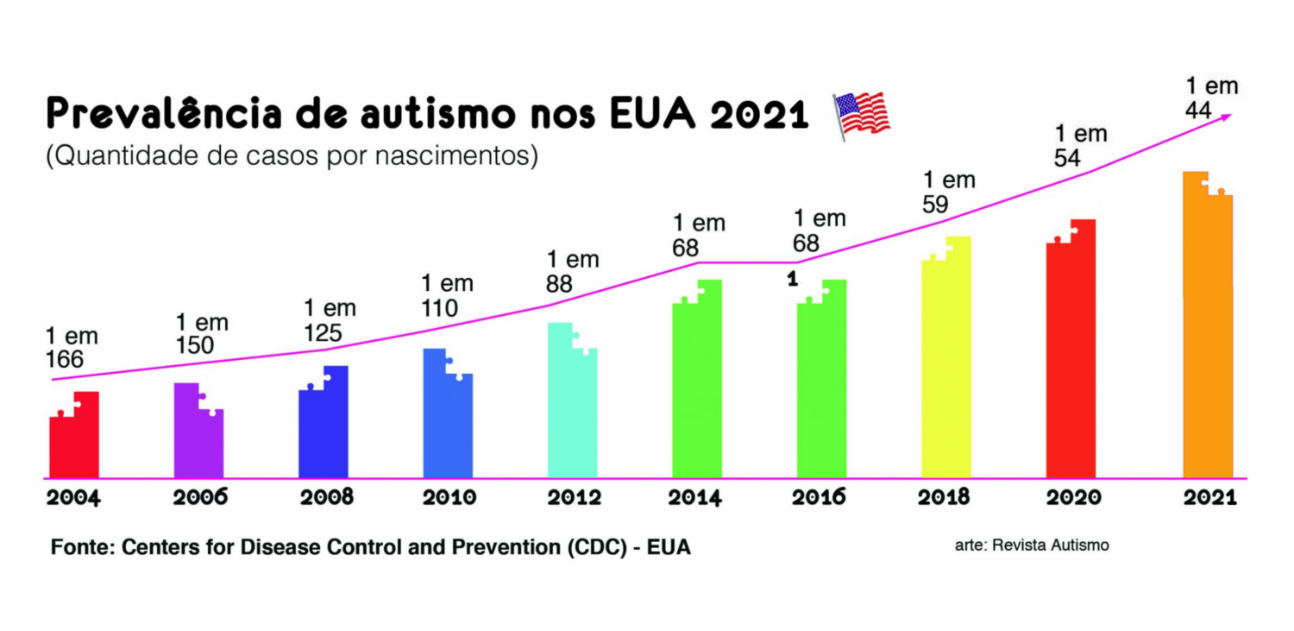
\includegraphics[width=0.9\textwidth]{anexos/diversaGenteGrafico.png}
\end{figure}

Tendo isso em mente, o diversaGente é um aplicativo destinado aos pais e mães de crianças Neurodiversas  pois é evidente que ter um filho com alguma neurodiversidade traz consigo vários desafios, como, por exemplo, encontrar escolas adequadas e um leque de profissionais especializados.

\section{Relato de usuário}

Conforme a concretização da ideia e o desenvolvimento do aplicativo avançaram, foi possível buscar um exemplo de aplicação real para um potencial usuário. Victoria Severiana, amiga do intregrante da equipe Gabriel Ruiz, é irmã de uma menina portadora da síndrome de Down e concordou em trazer um relato sobre a ideia e sobre o teste de uma versão beta do aplicativo.

"Em 2016, eu e meus pais soubemos que receberíamos uma criança com Síndrome de Down na família. Ainda na gestação, meus pais receberam a notícia e não souberam o que fazer com a informação, pois nunca tinham tido contato com nenhum portador ou parente. Inclusive, esconderam o fato por algumas semanas de mim (com 15 anos) e da minha outra irmã (com 10 anos), com medo de como lidaríamos com isso. Nesse momento, partindo do zero, eles se beneficiaram da facilidade da comunicação e da quantidade de informações encontradas na internet, buscando referências em fóruns, sites e grupos de redes sociais (GRAAC, APAE, Teleton, Grupo Pais de Crianças com Síndrome de Down do Facebook etc.). Depois do nascimento da minha irmã, Clara, também descobrimos que ela tinha uma doença cardíaca congênita, o que exigiu uma cirurgia de alto risco antes de 1 ano de idade. Outra condição que minha irmã também tem é a Paralisia de Bell. Todos esses fatos geraram ansiedade na família, que sempre buscou pelo melhor da Clara, e, sem dúvida, um app ou uma rede de apoio construída em torno de uma comunidade como o diversaGente teria facilitado muito os meios de chegar à informações úteis para o desenvolvimento dela. Hoje, já teríamos diversas recomendações para fazer dentro do app, sobretudo para círculos de crianças diversas na região Oeste de São Paulo: locais de terapia, a APAE de Cotia, estabelecimentos que são receptivos e adaptados a essas condições, tipos de alimentação, atividades lúdicas para desenvolvimento neural e motor etc., só para citar algumas coisas, pois conviver com uma criança diversa é aprender literalmente todos os dias."

Victoria Severiana da Silva, irmã da Clara, portadora da síndrome de Down.


E-mail para contato: victoriaseveriana@gmail.com


Telefone para contato: (11) 96329-1565


\section{Análise de concorrência}

A seção tem o intuito de, através de pesquisas na internet, traçar um comparativo de aplicativos com finalidades similares às do diversaGente e evidenciar as particularidades que esta tem em relação às outras. É possível ver no \autoref{tabela-comparativo} as características de cada aplicação para melhor visualização. 

O primeiro a ser comparado é o Facebook, além de ser uma das redes sociais mais usadas no Brasil e no mundo, possui algumas características similares com o diversaGente, como feed de postagem dentro de grupos, perfil pessoal e opção de compartilhamento de postagens. 

Para o Twitter, uma rede social que é um enorme fórum, muito utilizada entre os jovens, porém não possui nenhuma página para criar grupos e se conversar sobre um assunto específico. Possui um filtro bem eficiente que é possível buscar por algo, caso alguém já tenha feito uma postagem sobre. 

A Tismoo.me é a aplicação mais parecida com o diversaGente, possuindo também um fórum, nichada para o público de pais e responsáveis de crianças pertencentes ao espectro autista. O diversaGente consegue se diferenciar do Tismoo.me pelas funcionalidades de avaliação de locais, sendo possível compartilhar a experiência do usuário e também pela interação de chat em tempo real entre dois usuários. 

A característica principal da Emergency Chat é que pode ser utilizada em qualquer situação onde a fala é impossível, mas a comunicação ainda é necessária. Não é necessariamente uma rede social, possui um chat para comunicação.  

O TippyTalk é um aplicativo voltado para pais ou responsáveis de crianças neurodiversas, principalmente aquelas com alguma dificuldade de comunicação verbal. Permite que um administrador crie imagens exclusivamente identificáveis e familiares para as crianças, apoiando na educação e treino de atividades/tarefas rotineiras. 

O The Autism Helper também tem grande similaridade com o diversaGente porque é voltado para quem procura a facilitar, o máximo possível, a vida de indivíduos do espectro autista. O aplicativo possui fóruns para discussão e perfil pessoal. 



\
\begin{quadro}[thb]
	\centering
	\ABNTEXfontereduzida
	\caption[Comparativo entre aplicações]{Comparativo entre aplicações}	\label{tabela-comparativo}

	\begin{tabular}{|l|c|c|c|c|c|c|c|}
		\hline
		\thead{ } & \thead{diversa\\Gente} & \thead{Facebook}  & \thead{Twitter}  & \thead{Tismoo\\.me} & \thead{Emergency\\ Chat}  & \thead{Tippy\\ Talk}  & \thead{The \\Autism \\Helper}\\
		\hline
		Público Neurodiverso & X &  &  & X & X & X & X \\
		\hline
		Consultar Notícias & X &  & X & X &  &  &  \\
		\hline
		Fóruns & X & X &  & X &  &  & X \\
		\hline
		Locais Avaliados & X &  &  &  &  &  & \\
		\hline
		Chat & X & X & X &  & X & X &  \\
		\hline
		Feed de Postagem & X & X & X & X &  &  & X\\
		\hline
		Perfil Pessoal & X & X & X & X &  &  & \\
		\hline
		Buscar Usuários & X & X & X & X &  &  & \\
		\hline
		Compartilhar & X & X & X & X &  &  & X \\
		\hline
	\end{tabular}
\fonte{Equipe diversaGente (2022)}
\end{quadro}



% ---
% Capitulo de revisão de literatura
% ---
\chapter{Revisão da Literatura}

Neste tópico iremos fazer um estudo e tirar observações mais a fundo a respeito da neurodiversidade. Relatar quando começou os estudos a respeito das pessoas neurodiversas e
entender como foi o papel da sociedade no passado, no que nisso acarretou e as mudanças necessárias que surgiram para chegar nos dias de hoje.

\section{Influência do termo}
As questões neurodiversas em toda sociedade sempre foi um assunto difícil de falar, principalmente porque no passado era tratado com "modelo de tragédia pessoal" \cite{oliver1990politics}. Dessa maneira, foi crescendo o indiferente e inquestionável a respeito das pessoas que sofrem algum tipo de neurodiversidade. Entretanto, com os estudos, os teóricos que estudavam a causa mais fundo diziam que esse modelo social estaria equivocado, pois se deixar que essa percepção percorra nossa sociedade não irá trazer as necessárias responsabilidades sociais que devemos atingir para evitar esses equívocos. Sendo assim, essa mudança de responsabilidade para o comportamento com as neurodiversidades promove o empoderamentos do indivíduo e sendo assim ele ganha espaço para ser olhado pela sociedade e respeitado por elas.

\section{Virada de responsabilidades}
Um dos motivos que nos levou a trazer o tema da neurodiversidade para o projeto final está na maneira que o assunto é tratado na sociedade. Há muitos tabus a serem derrubados. Se, por volta de 1960, ainda se culpavam os pais pelos seus filhos terem nascido com alguma neurodiversidade e, portanto, impossibilitava o surgimentos de movimentos que pudessem entender e ajudar os familiares, hoje temos algumas conquistas a serem celebradas como projetos de leis que protejam as pessoas neurodiversas graças aos estudos sobre deficiência nos anos 70 que desconstruiu um modelo de responsabilidade única para uma socialmente construída.\cite{ortega2008}. Todavia, o preconceito, falta de informação e suporte ainda estão presentes no convívio social e dessa maneira, trazer uma rede social focada para sanar dúvidas e compartilhar informações e serviços torna-se esse assunto vivo diante a sociedade.

\section{Responsabilidade do Aplicativo}
Apontado no artigo de \cite{rios}, evidencia-se que no Brasil há um embate entre profissionais e pais a respeito do movimento neurodiverso, uma vez que a sociedade brasileira ainda está atrelada aos modelos ultrapassados lá da décadas de 1960. Dessa maneira, o diversaGente tem como objetivo tornar-se um ambiente de discussões e compartilhamento de informações sobre o assunto. Assim, o comprometimento na era digital que vivemos junto com a neurodiversidade nos remete ao compartilhamento de mais informações a respeito do assuntos com pessoas em diversos lugares, diversas famílias e culturas, pois em diversos artigos apresentam críticas a forma que os métodos atuais de tratamento são usados, uma vez que muitos tratamentos centram-se na deficiência e não na forma humana que deve ser tratado\cite{machado}. 


% ---


% Para facilitar a manutenção é sempre melhore criar um arquivo por capitulo, para exemplo isso não é necessário 
% Para facilitar a manutenção é sempre melhore criar um arquivo por capitulo, para exemplo isso não é necessário 

%---------------------------------------------------------------------------------------
\chapter{Escalabilidade}

O quesito ‘escalabilidade’ é muito abordado e de extrema importância atualmente, principalmente devido ao enorme fluxo de dados que corre dentre os sistemas e aplicações. A escalabilidade diz respeito a facilidade de crescimento da infraestrutura da aplicação de forma saudável, sem grandes impactos nos custos ferramentais e humanos e no desempenho da aplicação. Essa adaptabilidade pode estar relacionada com a implementação de novas funcionalidades, novas demandas de mercado, inserção em requisições legislativas e projetos de inovação, por exemplo. 

O projeto conta com ferramentas muito atuais, que já trazem consigo muito fortemente o conceito de escalabilidade, como o Heroku e o Docker, o primeiro que ganha cada vez mais espaço de mercado como uma Platform as a Service (PaaS), em que a solução permite que o desenvolvedor se desapegue de detalhes estruturais, trazendo maior facilidade de manutenção e maior agilidade de deploy, já o segundo possibilita a criação de ambientes virtuais completos, os chamados contêineres, que podem até mesmo ter seu crescimento automatizado de acordo com a demanda de requisições, gerando novos contêineres semelhantes, por exemplo. 

Por se tratar de um modelo de aplicação com pouca concorrência em mercado, existem chances relevantes de crescimento, assim, é possível que haja a necessidade de escalada da aplicação em um futuro breve, tendo isso em consideração, as ferramentas anteriormente citadas se encaixam muito bem nessa possível necessidade futura. 


%---------------------------------------------------------------------------------------
\chapter{Critérios de segurança}

\begin{itemize}
    \item A aplicação está de acordo com a Lei Geral de Proteção de Dados (LGPD, Lei nº13.709/2018). 
    
    \item Os dados que serão coletados e utilizados são: Como o usuário gostaria de ser chamado, foto do usuário opcional, data de nascimento, e-mail, neuroatipicidade da criança, localização aproximada opcional e senha. Não é obrigatório a publicação nem carregamento de dados pessoais que não queira disponibilizar ao público. 
    
    \item Para maior garantia de segurança, o armazenamento da senha será feito com criptografia e os dados dos usuários obterão total sigilo, sendo visíveis apenas pelo próprio usuário e por administradores do sistema em situações que sejam necessárias. 
    
    \item Os dados não sensíveis dos usuários (como nome de usuário e foto de perfil) serão visíveis para todos os usuários cadastrados, já dados sensíveis serão visualizáveis apenas pelo próprio usuário e, se necessário, pelos administradores da plataforma. 
    
    \item Os dados terão a sua integridade mantida, ou seja, não sofrerão alterações indevidas sem autorização do usuário, para que não possam vir a corromper a veracidade das informações. 
    
    \item Caso o usuário opte por encerrar sua conta, os seus dados pessoais não ficarão mais visíveis para outros usuários e seu perfil não deverá mais ser encontrado nas buscas dentro do aplicativo. Em 30 dias após o encerramento da conta todos os dados e informações da conta encerrada serão excluídos. 
\end{itemize}

%---------------------------------------------------------------------------------------
\chapter{Tecnologias a serem utilizadas}

Para o lado do cliente, iremos utilizar o React Native com Typescript junto a ferramenta Expo para testar o app com as APIs nativas do Android que essa ferramenta disponibiliza.

Já para o lado do servidor, utilizaremos Node.js com Typescript e framework NestJS para a construção da API, MongoDB como banco de dados, Prisma como ORM, Cloudinary como storage e para documentação de API, a especificação OpenAPI.

Para o ambiente de desenvolvimento, será utilizado o Docker a fim de obtermos facilidade em executar o projeto independente do Sistema Operacional local.

A hospedagem se dará por meio da Play Store para o app em React Native, do Heroku para o backend em Node.js e do MongoDB Atlas para o banco de dados.
Todo o versionamento será feito por meio das plataformas Github e Subversion.

Para realizar a prototipação das interfaces, será utilizada a ferramenta Figma e a construção de fluxos e brainstorms da equipe se darão por meio do Miro e Whimsical.

Por fim, para o gerenciamento do projeto, utilizaremos o Trello para registro de backlog e acompanhamento do status de desenvolvimento das histórias, o Discord para realização das cerimônias semanais da equipe e o WhatsApp para comunicações rápidas e mais urgentes entre o time.

\chapter{Manutenibilidade da aplicação desenvolvida}

\section{Ferramentas compatíveis com as tecnologias escolhidas para Testes automatizados e Análise Estática}
Usaremos Jest, um framework JavaScript para testes automatizados, e ESLint para análise estática do código.

\section{Sistemas de log para toda a aplicação}
Papertrail será o sistema de log que utilizaremos para mapear o comportamento da API em Node.js.

\section{Um processo de Integração Contínua}
A partir das Github Actions iremos estabelecer nosso workflow de CI (Continuous Integration).

\section{Especificação do “Coding Convention” (seja o próprio da linguagem, ou um criado/adaptado pela equipe)}
Usaremos o padrão recomendado pelo próprio ESLint para adequar:
\begin{itemize}
    \item Layout e formatação;
    \item Sugestão de alternativas para implementação do código (como, por exemplo, o uso do padrão camelCase para nomenclatura);
    \item Regras que visam corrigir possíveis problemas de lógica do código.
\end{itemize}
Todas as especificações a serem utilizadas estão disponíveis em: https://eslint.org/docs/rules/

\section{Design Patterns pertinentes à aplicação}
Utilizaremos os padrões Observer, Singleton e Injeção de Dependência.

\chapter{Diagrama de classes do sistema}
\begin{sidewaysfigure}[htb]

    \centering
	\caption{\label{fig_diag_virado}Diagrama de classes do sistema}
	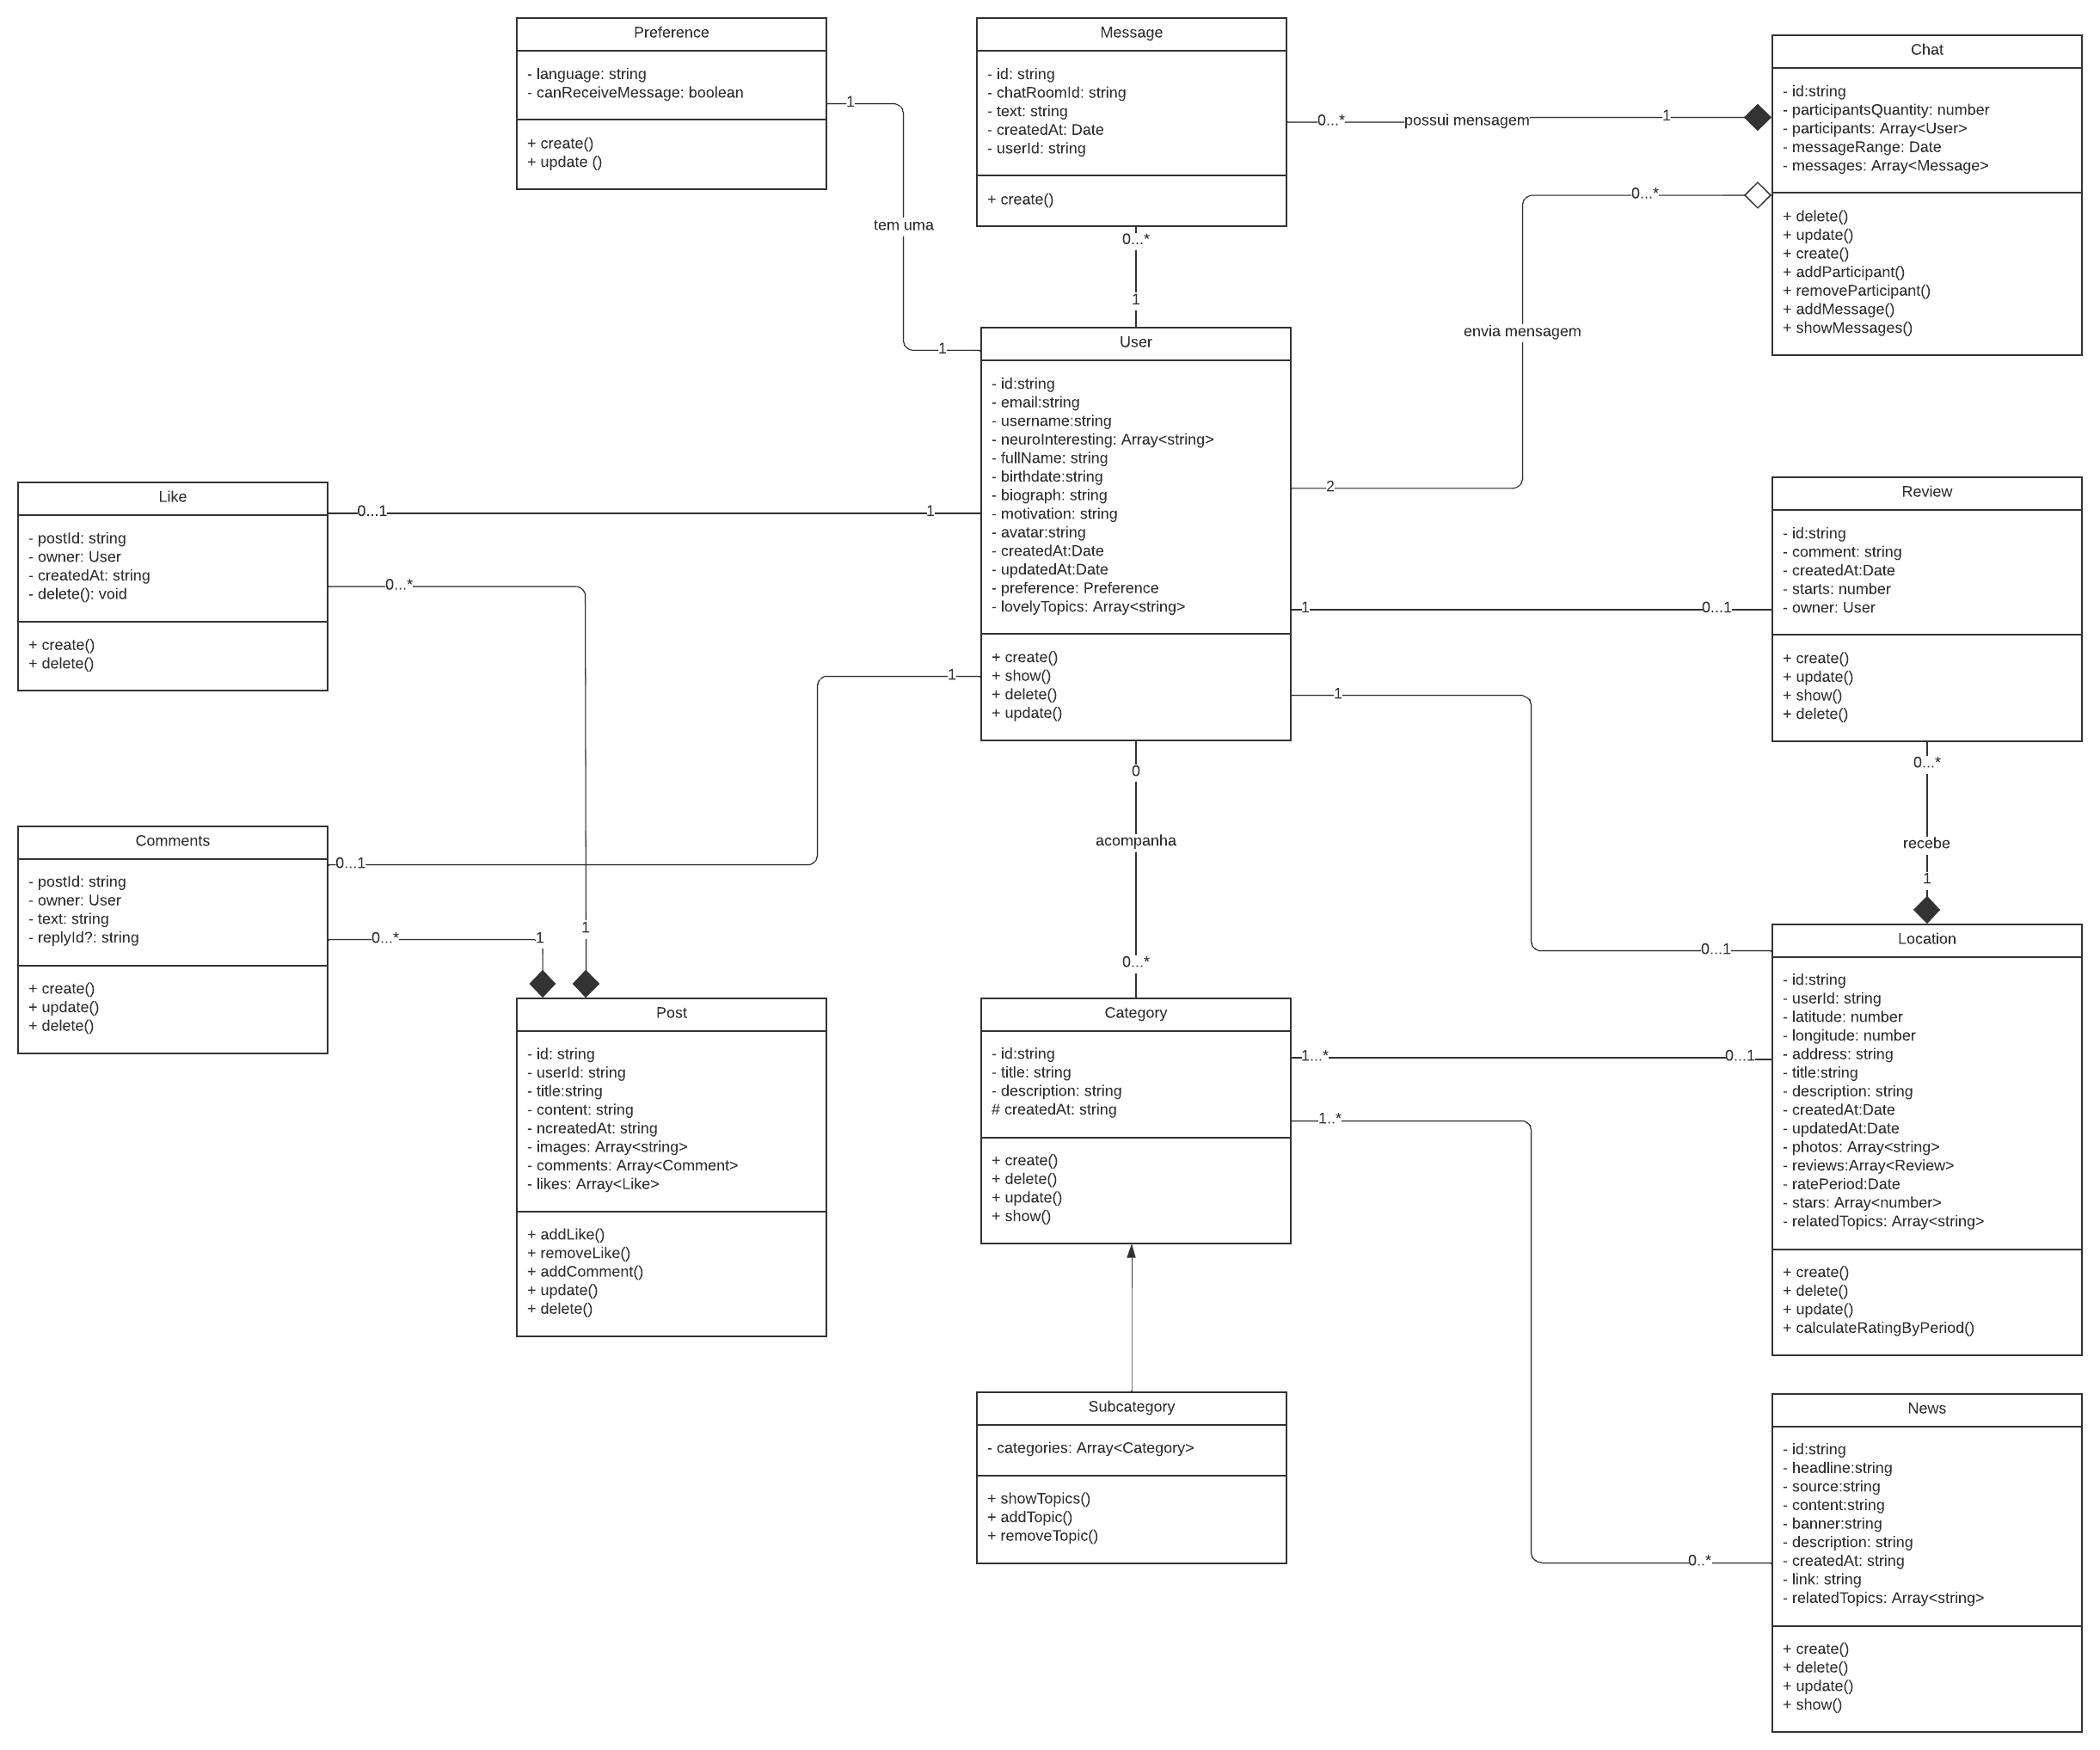
\includegraphics[width=0.9\textwidth]{anexos/diagrama.png}

	\end{sidewaysfigure}
%---------------------------------------------------------------------------------------





% exemplos de escrita LaTeX
\chapter{Exemplos \LaTeX}
\label{cap-exemplos}

\explicacao{ATENÇÃO : Este capítulo e os seguintes demonstram como fazer no {\LaTeX} portanto devem ser lidos em conjunto com o código fonte desse documento}

% exemplo de como inserir uma referencia adicional no sumario (normalmente não utilizado em um trabalho acadêmico)
\addcontentsline{toc}{chapter}{Exemplos que devem ser lidos (mas esse tipo de indicação não vai em um trabalho acadêmico) :-)}

Esse capítulo tem exemplos de escrita utilizando o {\LaTeX}  utilizando \abnTeX, é muito simples escrever em \textbf{negrito}, \textit{itálico} \footnote{apesar de que nesse documento \mostraComandoLaTeX{textit} \mostraComandoLaTeX{emph} tem comportamento parecido é recomendável utilizar \mostraComandoLaTeX{textit} de forma genérica para itálico}, ....


Existem diversos tutoriais para uso de \LaTeX, se você está utilizando esse modelo não precisará se preocupar com muitos dos detalhes técnicos do \LaTeX \space e cuidar somente do seu texto.

Escolha seu editor : \url{https://en.wikipedia.org/wiki/Comparison\_of\_TeX\_editors}, apesar do overleaf sem bem prático, nem todas as funções estão disponíveis na versão gratuita e você pode instalar gratuitamente em seu computador um compilador \LaTeX \space e utilizar um sistema de controle de versão para gerenciar seu documento.


\section{Normas ABNT}

Esse documento modelo já resolve boa parte da padronização NBR 14.724:2011 \cite{NBR14724:2011} que deve ser seguida e inclusive alguns pontos que não são claros pelo modelo de padronização do \ac{ifsp}.

Leia os documentos do {\abnTeX} e do \ac{ifsp}:
\begin{itemize}
    \item \url{https://www.abntex.net.br/}
    
    \item \acs{faq} : \url{https://github.com/abntex/abntex2/wiki/FAQ}
    
    \item \url{http://mirror.unl.edu/ctan/macros/latex/contrib/abntex2/doc/abntex2.pdf}
    
    \item \waUrl{https://spo.ifsp.edu.br/biblioteca?id=184}
\end{itemize}

No \ac{ifsp} você pode acessar todas as normas \ac{abnt} sem custo, as informações estão disponíveis no endereço \waUrl{https://www.ifsp.edu.br/index.php/outras-noticias/52-reitoria/2329-alunos-e-servidores-do-ifsp-podem-acessar-abnt-via-web.html}.

Apesar de alguns elementos serem opcionais na \ac{abnt} eles foram definidos como obrigatórios (folha de rosto, resumo, lista de siglas, lista de ilustrações, glossário etc), nos trabalhos completos de projetos de informática do \ac{ifsp} campus São Paulo. Documentos menores como propostas de projeto, documento de \ac{poc} não necessitam desses elementos, mas alguns podem ser uteis para ajudar no estudo do {\LaTeX} em preparação para o documento final.

\begin{itemize}
    \item Logotipo da instituição, não é citado na \ac{abnt} nem no manual de normalização do \ac{ifsp}, mas aparece em uma imagem do documento de normalização, foi definido que não deve ser incluído na capa;
    
    \item Nome da instituição que é opcional na capa, deve ser utilizado;
    
\end{itemize}



\section{Detalhes textuais}

O documento é dividido em capítulos, e cada capítulo dividido em seções utilizando o \abnTeX \space você pode dividir seus documentos nos níveis de acordo com os comandos:

\begin{itemize}
    \item \mostraComandoLaTeX{chapter}  (1);
    
    \item \mostraComandoLaTeX{section} (1.1);
    
    \item \mostraComandoLaTeX{subsection} (1.1.1);
    
    \item \mostraComandoLaTeX{subsubsection} (1.1.1.1);
    
    \item \mostraComandoLaTeX{subsubsubsection} (1.1.1.1.1).
    
\end{itemize}

Tenha em mente que normalmente se utiliza no máximo o nível \mostraComandoLaTeX{subsection}.
Ao definir as divisões do seu trabalho utilizando as diretivas do \LaTeX, elas são automaticamente inseridas no sumário do documento.


\subsection{Caracteres Reservados e auxiliares}



Alguns caracteres são reservados no \LaTeX \space e por isso para utilizar esses caracteres é necessário utilizar uma forma diferenciada de escrita. É possível utilizar a macro \mostraComandoLaTeX{symbol} com o código \ac{ascii} do caracter desejado, veja no código fonte desse texto como utilizar corretamente esses itens.


\begin{itemize}
\item barra invertida : \textbackslash   \symbol{92}    $\backslash$;
\item til  :  \symbol{126} ;
\item cifrão : \$;
\item sublinhado, \textit{underscore}, \textit{underline} : \_;
\item \enquote{aspas} as macros \mostraComandoLaTeX{enquote} / \mostraComandoLaTeX{textquote} garantem o espaçamento correto, se utilizar diretamente as ASPAS o espaçamento é perdido;
% https://tex.stackexchange.com/questions/80395/no-space-after-closing-double-quote
\item marcadores : \cmark\ \xmark\ \circlemark\ \ding{100} \ - ver mais no \refanexo{pifont-quickref};
\item chaves : \} \{.
\end{itemize}

\subsection{Listas}

Em uma lista de itens cada item deve ser terminado por ponto e virgula, exceto o ultimo item que deve ter um ponto final.

\begin{itemize}
\item item 1;
\item item 2;
\item item ..;
\item item final.
\end{itemize}


\subsection{Citações / Referências}
\label{referencias}

Em um trabalho acadêmico você deve buscar referencias que servem de base para seus estudos, essas referencias devem ser confiáveis, normalmente artigos e livros são confiáveis pois passam por um processo de revisão por especialistas na área. É importante buscar as referencias primárias e não utilizar a informação escrita por outra pessoa (referencia secundária). As citações são definidas pela \citetitle{NBR10520:2002} e as referencias pela \citetitle{NBR6023:2018}, sendo interessante observar que a \citeonline{NBR6023:2018_alteracoes} fez uma resumo com algumas das mudanças ocorridas em 2018.


A \ac{abnt} define a citação da citação (\textit{apud}), mas sua utilização não deve ser feita exceto em casos onde o documento original não possa ser acessado de nenhuma forma. Atualmente a maioria dos documentos se encontra disponível de forma digital o que permite a busca das informações em suas fontes primárias de forma que o \textit{apud} não é bem visto. 

Não é indicada a utilização de sites como Wikipedia como fonte de informações pois a Wikipedia é uma referencia secundária, já que exige que seus artigos tenham referencias da informação, e com isso a utilização da Wikipedia cai no mesmo caso da utilização de \textit{apud} indicada anteriormente, já que é possível buscar a informação diretamente na fonte primária.

Quando for necessário citar sites deve ser utilizada a ferramenta \url{https://web.archive.org}, caso não exista uma referencia salva anteriormente basta salvar e utilizar. O uso dessa ferramenta muitas vezes ajuda também a determinar a data estimada de publicação de informação quando o site já foi salvo anteriormente e não possui data de publicação disponível.



Existem diversas formas de citação que devem ser escolhidas de acordo com o contexto do texto onde são utilizadas, observe os exemplos :

\begin{itemize}
    \item \mostraComandoLaTeX{cite} - utilizada normalmente em final de paragrafo: \newline
    \cite{UML:JACOBSON} | \cite{POWELL:2006} \\ 
        \cite{SCRUMGUIDE:2013} | \cite{urani1994} |\\
        \cite{ETAL5} | \cite{ETAL4}; 
    
    \explicacao{Se as duas ultimas referencias aparecem somente com um autor, você está compilando o documento com uma versão antiga do \mostraPacoteLaTeX{abntexcite}, o overleaf em 2021-07-06 estava desatualizado}
    \explicacao{ABNT 6023:2018 8.1.1.2 recomenda para utilizar TODOS autores sempre, mas permite utilizar et al, dependendo da versão do \mostraPacoteLaTeX{abntexcite} isso não está acontecendo corretamente}

    \item \mostraComandoLaTeX{citeonline}  - utilizada normalmente em textos como \enquote{(segundo|de acordo| com) ...}: \newline
    \citeonline{UML:JACOBSON} | \citeonline{POWELL:2006} \\
        \citeonline{SCRUMGUIDE:2013} | \citeonline{urani1994} \\
        \citeonline{ETAL5} | \citeonline{ETAL4};

    \item \mostraComandoLaTeX{citeauthoronline} - raramente utilizado, quando se deseja citar somente o autor: \newline
    \citeauthoronline{UML:JACOBSON}| \citeauthoronline{POWELL:2006} \\
        \citeauthoronline{SCRUMGUIDE:2013} | \citeauthoronline{urani1994} \\
        \citeauthoronline{ETAL5} | \citeauthoronline{ETAL4};

    \item \mostraComandoLaTeX{citeauthor} - muito pouco utilizado: \newline \citeauthor{UML:JACOBSON}| \citeauthor{POWELL:2006} \\
        \citeauthor{SCRUMGUIDE:2013}| \citeauthor{urani1994} \\
        \citeauthor{ETAL5} | \citeauthor{ETAL4};
    
    \explicacao{Se as duas ultimas referencias aparecem somente com um autor, você está compilando o documento com uma versão antiga do \mostraPacoteLaTeX{abntexcite}, o overleaf em 2021-07-06 estava desatualizado}

    \item \mostraComandoLaTeX{citetitle} - muito pouco utilizado: \newline
    \citetitle{UML:JACOBSON}|\citetitle{POWELL:2006} \\
        \citetitle{SCRUMGUIDE:2013}| \citetitle{urani1994} 
        
    \explicacao{O comando \mostraComandoLaTeX{citetitle} está disponível utilizando a biblioteca \mostraPacoteLaTeX{biblatex}}

\end{itemize}

A documentação do abntex2cite possui muitos exemplos de como utilizar corretamente cada formato de citação : \url{https://mirrors.ibiblio.org/CTAN/macros/latex/contrib/abntex2/doc/abntex2cite-alf.pdf}.

Cada formato de citação deve ser utilizado em um contexto especifico :
\begin{itemize}
    \item De acordo com \citeonline{SCRUMGUIDE:2013} .....;
    
    \item Fonte: \citeonline{SCRUMGUIDE:2013};
    
    \item sua explicação de um assunto baseado em uma referência \cite{SCRUMGUIDE:2013}.
    
\end{itemize}

ATENÇÃO : Alguns parâmetros de formatação foram alterados em 2018, mas não foram corrigidos ainda nos pacotes do \ac{abntex}, devem ser alterados manualmente ou utilizar as versões de desenvolvimento
\begin{itemize}
    \item \url{https://github.com/abntex/abntex2/issues/210}
    
    \item \url{https://github.com/abntex/biblatex-abnt/issues/42}
\end{itemize}

Os dados devem ser definidos corretamente nos arquivos \textquote{.bib} para a correta formatação no texto e na lista de referências.

Para autor com diversas publicações no mesmo ano : são geradas letras automaticamente pelo compilador de acordo com a ordem que são apresentadas na bibliografia, a letra não aparece na lista de referencias. \footnote{\url{https://github.com/abntex/biblatex-abnt/issues/20}}




\subsection{Abreviaturas / Siglas / Glossário}
\label{siglas-glossario}

Palavras que devem ser apresentadas no glossário devem ser citadas especificamente no texto utilizando os comandos de glossário como : \gls{tag}. Nesse modelo as definições de glossário devem ser feitas no arquivo \textbf{defs-glossario.tex}.

As abreviaturas nesse modelo devem ser feitas no arquivo \textbf{defs-siglas.tex}, tomando o cuidado de definir corretamente as siglas de outras línguas e as da língua portuguesa. Abreviaturas normalmente são referenciadas utilizando \mostraComandoLaTeX{ac}, mas podem ser referenciadas diretamente na versão reduzida \textquote{\acs{ifsp}} (\mostraComandoLaTeX{acs}) \space  
ou longa \textquote{\acl{ifsp}} (\mostraComandoLaTeX{acl}).

Na primeira vez que a sigla aparecer no texto o compilador {\LaTeX} mostra por extenso e a partir dai mostra somente a sigla:

\begin{itemize}
    \item \ac{se}
    
    \item \ac{se}
    
\end{itemize}

Quando uma sigla é utilizada em titulo de figura ela não deve aparecer por extenso. A maneira correta para que isso aconteça é utilizar a sigla com \mostraComandoLaTeX{acs} no titulo da figura como apresentado na \autoref{fig_sge1} pela sigla \ac{sge1}.

\begin{figure}[hb]
    \centering
	\caption{\label{fig_sge1}Exemplo de sigla em titulo de ilustração \acs{sge1}}
    \missingfigure[figwidth=6cm]{Exemplo para uso de sigla em titulo \ldots}	
	\fonte{Os autores.}
\end{figure}



Lembre que o {\LaTeX} tem vários passos de compilação, sempre que alterar as chamadas de siglas / referencias é recomendável uma compilação completa do documento.








\subsection{Elementos não textuais / Ilustrações}
\label{elementos-nao-textuais}

Elementos não textuais são aqueles que auxiliam o entendimento, não podem ficar \enquote{jogados} no texto, devem ser citados, cada elemento deve ser identificado por um \mostraComandoLaTeX{label} único que permite a sua referencia, no texto utilizando \mostraComandoLaTeX{ref} ou \mostraComandoLaTeX{autoref}, esses elementos quando definidos corretamente também são inseridos nas listas presentes antes do sumário.

Cuidado com o artigo \textbf{O/A} antes da Figura, Tabela ou Quadro referenciado, deve ser compatível com o tipo da ilustração.

Lembre que o \LaTeX \  vai posicionar os elementos  da melhor maneira possível dentro do documento, sempre faça as referencias utilizando os comandos específicos, nunca utiliza \enquote{acima}, \enquote{"baixo}, \enquote{a seguir}, etc... 

O posicionamento desses elementos é feito pelas rotinas do pacote float, leia a documentação em  \url{http://linorg.usp.br/CTAN/macros/latex/contrib/float/float.pdf}. É recomendável utilizar as opções de posicionamento \textbf{htb}, a opção \textbf{H} deverá ser utilizada somente como ultima alternativa de posicionamento e em alguns casos a utilização de \mostraComandoLaTeX{FloatBarrier} pode também melhorar o resultado se utilizada com cuidado.

Lembre que se houver uma grande distancia entre a ilustração no documento \ac{pdf} e sua definição original no documento isso significa que existe muito pouco texto em seu documento e isso não oferece muitas opções para o {\LaTeX} organizar as ilustrações. Você precisa nesse caso melhorar a descrição textual das ilustrações.


Para casos onde existe uma grande distancia entre a ilustração e o ponto de referencia no texto esse modelo possui macros \mostraComandoLaTeX{autorefwithpage} e \mostraComandoLaTeX{autorefwithpagedistance} a primeira sempre indica página onde a ilustração foi colocada e a segunda somente se a ilustração estiver mais distante que o número de páginas indicado como parâmetro, Ex. \autorefwithpage{fig_logo_A3}. Isso deve ser utilizado somente quando existe mais de uma referencia para mesma ilustração e não para deixar a ilustração distante de uma única referencia.

O titulo da ilustração deve ser apresentado sempre no topo (conforme \citetitle{NBR14724:2011}, era na parte inferior na  \citetitle{NBR14724:2005}), e a fonte deve ficar na parte inferior \cite{NBR14724:2011}. A norma não possui um exemplo direto do uso das fontes e é possível encontrar exemplos com e sem ponto final nas fontes das ilustrações. Considerando a utilização de ponto no manual do \ac{ibge} nesse modelo foi escolhido utilizar o ponto final na fonte das ilustrações.





% ---
\subsection{QR-Code}
% ---
\index{qr-code}
A utilização de códigos \ac{qr} facilita o acesso de endereços da internet a partir de dispositivos móveis com câmera.
As figuras \ref{qr-url-1} e \ref{qr-url-2} demonstram dois exemplos de endereços apresentados com essa tecnologia.


Para facilitar a utilização dos códigos \ac{qr}, deve-se tomar cuidado para não deixa-los alinhados na vertical pois dificulta a seleção a partir da câmera no dispositivo móvel.

Um exemplo para utilização de mais códigos de barra pode ser visto em : \urlmodelo.

Atenção, alguns compiladores podem ter problemas em utilizar a biblioteca \textbf{pstricks} necessária para gerar QR-Codes, no sharelatex em 2017-05 a compilação ocorre perfeitamente utilizando a opção de compilador "XeLatex", ele é mais lento que outras opções.


\begin{figure}
\begin{pspicture}(25mm,25mm)
\psbarcode{\urlmodelosimples}{eclevel=H width=1.0 height=1.0}{qrcode}
\end{pspicture}
\caption{\label{qr-url-1}QR-Code - URL Documento exemplo}
\legend{\urlmodelo}
\fonte{Os Autores}
\end{figure}



% colocando figura qrcode na direita para facilitar o uso da camera deixando cada qrcode em um alinhamento diferente
% se deixar os dois qrcodes um em cima do outro dificulta acessar o desejado
\begin{figure}
\begin{flushright}
\begin{pspicture}(25mm,25mm)
\psbarcode{https://github.com/ivanfmartinez/latexlib/tree/master/ifsp}{eclevel=H width=1.0 height=1.0}{qrcode}
\end{pspicture}
\caption{\label{qr-url-2}QR-Code - Classes IFSP GitHub}
\legend{\url{https://github.com/ivanfmartinez/latexlib/tree/master/ifsp}}
\fonte{Os Autores}
\end{flushright}

\end{figure}


\subsection{Organizando pendências}

Durante o desenvolvimento de um trabalho escrito é normal que alguns elementos sejam gerados posteriormente, mas é importante se organizar para não esquecer de fazer os ajustes necessários. Para isso recomendo a utilização do pacote \textbf{todonotes} que oferece diversos recursos para gerar lembretes das pendencias. O manual do \textbf{todonotes} está disponível no \autoref{manual-todonotes}\footnote{observe que existe um erro nesse documento, já que a referencia deveria ser Anexo e aparece como Apêndice,  existe um \textit{bug} no abntex2 ao referenciar anexos, para fazer corretamente veja \url{https://github.com/abntex/abntex2/issues/76} e utilize \mostraComandoLaTeX{refanexo} que está disponível nesse modelo.}.

É possível fazer anotações de pendencias inclusive indicando as pessoas responsáveis por elas, % nao mover o todo pois foi feito no meio do paragrafo exatamente para demonstrar um possível problema de formato
\todo[inline,author=Pessoa1]{fazer revisão das imagens do texto} e para facilitar a visualização criar imagens que funcionam como marcadores para figuras que serão incluídas posteriormente.

Cuidado ao utilizar as anotações \textit{inline} pois o texto ficara quebrado, como no paragrafo anterior.


\begin{figure}[htb]
    \centering
	\caption{\label{fig_todo1}Imagem que ainda não foi gerada}
	\missingfigure[figwidth=10cm]{você está atrasado pois ainda não criou esta figura}
	\fonte{dados do Projeto.}
\end{figure}



\subsection{Tabelas e Quadros}
\label{tabelas-e-quadros}
Quadros e Tabelas são informações tabulares, mas Tabelas tem como objetivo apresentar números. A ‘norma’ 14724 \cite[3.32]{NBR14724:2011} define a Tabela como sendo uma \enquote{forma não discursiva de apresentar informações das quais o dado numérico se destaca como informação central} e que devem seguir padronização do \ac{ibge}  \cite[5.9]{NBR14724:2011}. O \ac{ibge} padronizou a apresentações de dados tabulares em 1993 \cite{tabular-ibge}.

Informações adicionais sobre o de tabelas no {\LaTeX} podem ser obtidas em  \url{https://en.wikibooks.org/wiki/LaTeX/Tables}.

Antes de utilizar \index{longtable}\textbf{longtable} procure reorganizar o seu layout ou quebrar manualmente em múltiplos quadros / tabelas, pois isso ainda facilita a compreensão pelo leitor.

% https://biblioteca.ibge.gov.br/visualizacao/livros/liv23907.pdf

\index{quadros}O \autoref{quadro-exemplo} é um exemplo de dados tabulares gerados em 
\LaTeX.



\begin{quadro}[htb]
\centering
\ABNTEXfontereduzida
\caption[Níveis de investigação]{Níveis de investigação}
\label{quadro-exemplo}
\begin{tabular}{|p{2.6cm}|p{6.0cm}|p{2.25cm}|p{3.40cm}|}
  \hline
   \thead{Nível de\\Investigação} & \thead{Insumos}  & \thead{Sistemas de\\ Investigação}  & \thead{Produtos}  \\
    \hline
    Meta-nível & Filosofia\index{filosofia} da Ciência  & Epistemologia &
    Paradigma  \\
    \hline
    Nível do objeto & Paradigmas do metanível e evidências do nível inferior &
    Ciência  & Teorias e modelos \\
    \hline
    Nível inferior & Modelos e métodos do nível do objeto e problemas do nível inferior & Prática & Solução de problemas  \\
   \hline
\end{tabular}
\fonte{O Autor.}
\end{quadro}



\index{tabelas}Já a \autoref{tab-exemplo} foi criada conforme o padrão \citeonline{tabular-ibge} requerido pelas normas da \ac{abnt} para documentos técnicos e acadêmicos. Observe que não existem bordas laterais e nem linhas separadoras em uma Tabela e as colunas numéricas tem alinhamento à direita. 

\begin{table}[htb]
\centering
\caption{Métricas de desenvolvimento}
\label{tab-exemplo}
\begin{tabular}{p{2.6cm}rrr}
    \hline
   \thead{Item} & \thead{Janeiro}  & \thead{Fevereiro}  & \thead{Março}  \\
    \hline
    Classes & 2  & 10 & 20  \\
    Linhas & 100  & 250 & 543 \\
    \hline
\end{tabular}
\fonte{Os autores.}
\end{table}

\def\equationautorefname~#1\null{%
  Equação~(#1)\null
}


Para facilitar a criação de tabelas e quadros existem algumas ferramentas como o Tables Generator \url{http://www.tablesgenerator.com/latex_tables} que permite a criação de forma visual gerando o código \LaTeX\ correspondente. E o site \url{https://www.latex-tables.com/} permite converter planilhas em código \LaTeX.


\index{equação}\index{Pitágoras}A \autoref{eq-pythagoras} demonstra que também é possível escrever equações diretamente em \LaTeX

\begin{equation}\label{eq-pythagoras}
a^2+b^2=c^2\,.
\end{equation}






% ---
\subsection{Figuras}
\label{sec_figuras}
% ---

\index{figuras}Figuras podem ser criadas diretamente em \LaTeX,
como o exemplo da \autoref{fig_circulo}, ou inseridas a partir de arquivos externos como a \autoref{fig_logo}, que é o Logotipo do \ac{ifsp}. \index{logotipo}

% Aqui foi utilizada uma figura unica para demostrar a diferença de qualidade entr e vetorizado e não vetorizado pois fica mais simples, já que cada leitor pode ver esse documento em monitores com diferentes qualidades...
As figuras externas devem possuir boa qualidade e preferencialmente serem vetorizadas para se obter o melhor resultado. A \autoref{fig:nao_vetorizado_e_vetorizado} apresenta duas versões de uma mesma imagem demonstrando a variação de qualidade que pode acontecer quando não for utilizada a versão vetorizada, quando a figura possui elementos textuais pode até inviabilizar a leitura. As Figuras \ref{fig:uml_dia_nao_vetorizado_jpeg}, \ref{fig:uml_dia_vetorizado_eps} e \ref{fig:uml_dia_vetorizado_svg} foram reduzidas propositalmente no documento para demonstrar a diferença entre os formatos de arquivo. A diferença fica mais perceptível quando o documento é impresso ou quando existem textos pequenos e é necessário fazer zoom para visualização.

Procure criar suas imagens e diagramas pensando em utilizar impressão em preto-e-branco ou escala de cinza. Isto é importante, principalmente quando se pretende publicar o trabalho, uma vez que a maioria das publicações são somente em preto-e-branco. Outro benefício é o custo de impressão, normalmente menor para páginas preto-e-branco em relação a páginas coloridas.

Para diagramas em \ac{uml} o PlantUML pode ser utilizado para gerar código {\LaTeX} como exemplo na  \autoref{diagramauml}.


Se não houver a possibilidade de utilização de uma imagem vetorizada e existem diversos detalhes utilize \ac{png} em vez de \gls{jpg} ou outros formatos de menor qualidade, observe as diferenças nos exemplos apresentados em :  \waUrlTitle{https://tex.stackexchange.com/questions/136087/selecting-best-file-extension-for-graphics-figures-pictures}{Selecting best file extension for graphics figures pictures}.


\begin{figure}[htb]
	\caption{\label{fig_circulo}A delimitação do espaço}
	\begin{center}
	    \setlength{\unitlength}{5cm}
		\begin{picture}(1,1)
		\put(0,0){\line(0,1){1}}
		\put(0,0){\line(1,0){1}}
		\put(0,0){\line(1,1){1}}
		\put(0,0){\line(1,2){.5}}
		\put(0,0){\line(1,3){.3333}}
		\put(0,0){\line(1,4){.25}}
		\put(0,0){\line(1,5){.2}}
		\put(0,0){\line(1,6){.1667}}
		\put(0,0){\line(2,1){1}}
		\put(0,0){\line(2,3){.6667}}
		\put(0,0){\line(2,5){.4}}
		\put(0,0){\line(3,1){1}}
		\put(0,0){\line(3,2){1}}
		\put(0,0){\line(3,4){.75}}
		\put(0,0){\line(3,5){.6}}
		\put(0,0){\line(4,1){1}}
		\put(0,0){\line(4,3){1}}
		\put(0,0){\line(4,5){.8}}
		\put(0,0){\line(5,1){1}}
		\put(0,0){\line(5,2){1}}
		\put(0,0){\line(5,3){1}}
		\put(0,0){\line(5,4){1}}
		\put(0,0){\line(5,6){.8333}}
		\put(0,0){\line(6,1){1}}
		\put(0,0){\line(6,5){1}}
		\end{picture}
	\end{center}
	\fonte{Modelo Canônico ABNTeX2.}
\end{figure}


\begin{figure}[htb]
    \centering
	\caption{\label{fig_logo}Logotipo \ac{ifsp}}
	
\includegraphics{\ifspprefixo/logo-02.jpg}
	\fonte{\ac{ifsp}.}
\end{figure}

\begin{figure}
    \centering
    \caption{Exemplo de imagem não vetorizada e vetorizada}
    \label{fig:nao_vetorizado_e_vetorizado}
	
\includegraphics[width=0.95\textwidth]{erros/exemploVetorizacao.png}
    \fonte{\citeonline{vetorizacao}.}
\end{figure}
    

% Essas imagens foram reduzidas na apresentação para demonstrar o efeito da alteração de escala em imagens não vetorizadas
\begin{figure}
    \centering
    \caption{Exemplo de diagrama - salvo em imagem não vetorizada - JPEG}
    \label{fig:uml_dia_nao_vetorizado_jpeg}
	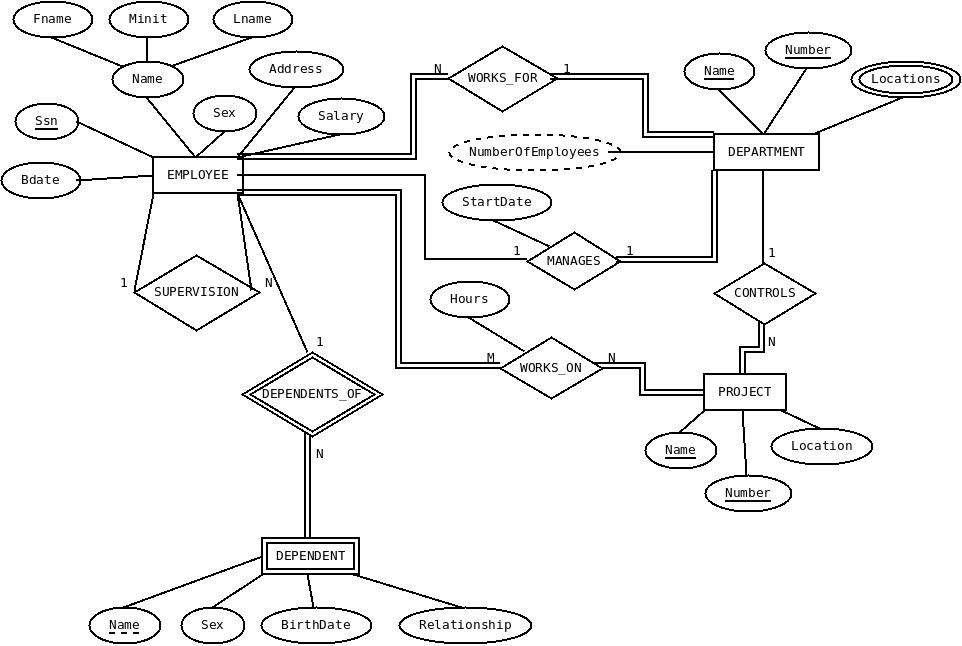
\includegraphics[width=0.6\textwidth]{exemplos/diagramas/ER.jpeg}
    \fonte{Indicar autor original.}
\end{figure}


\begin{figure}
    \centering
    \caption{Exemplo de diagrama - salvo imagem vetorizada - EPS}
    \label{fig:uml_dia_vetorizado_eps}
	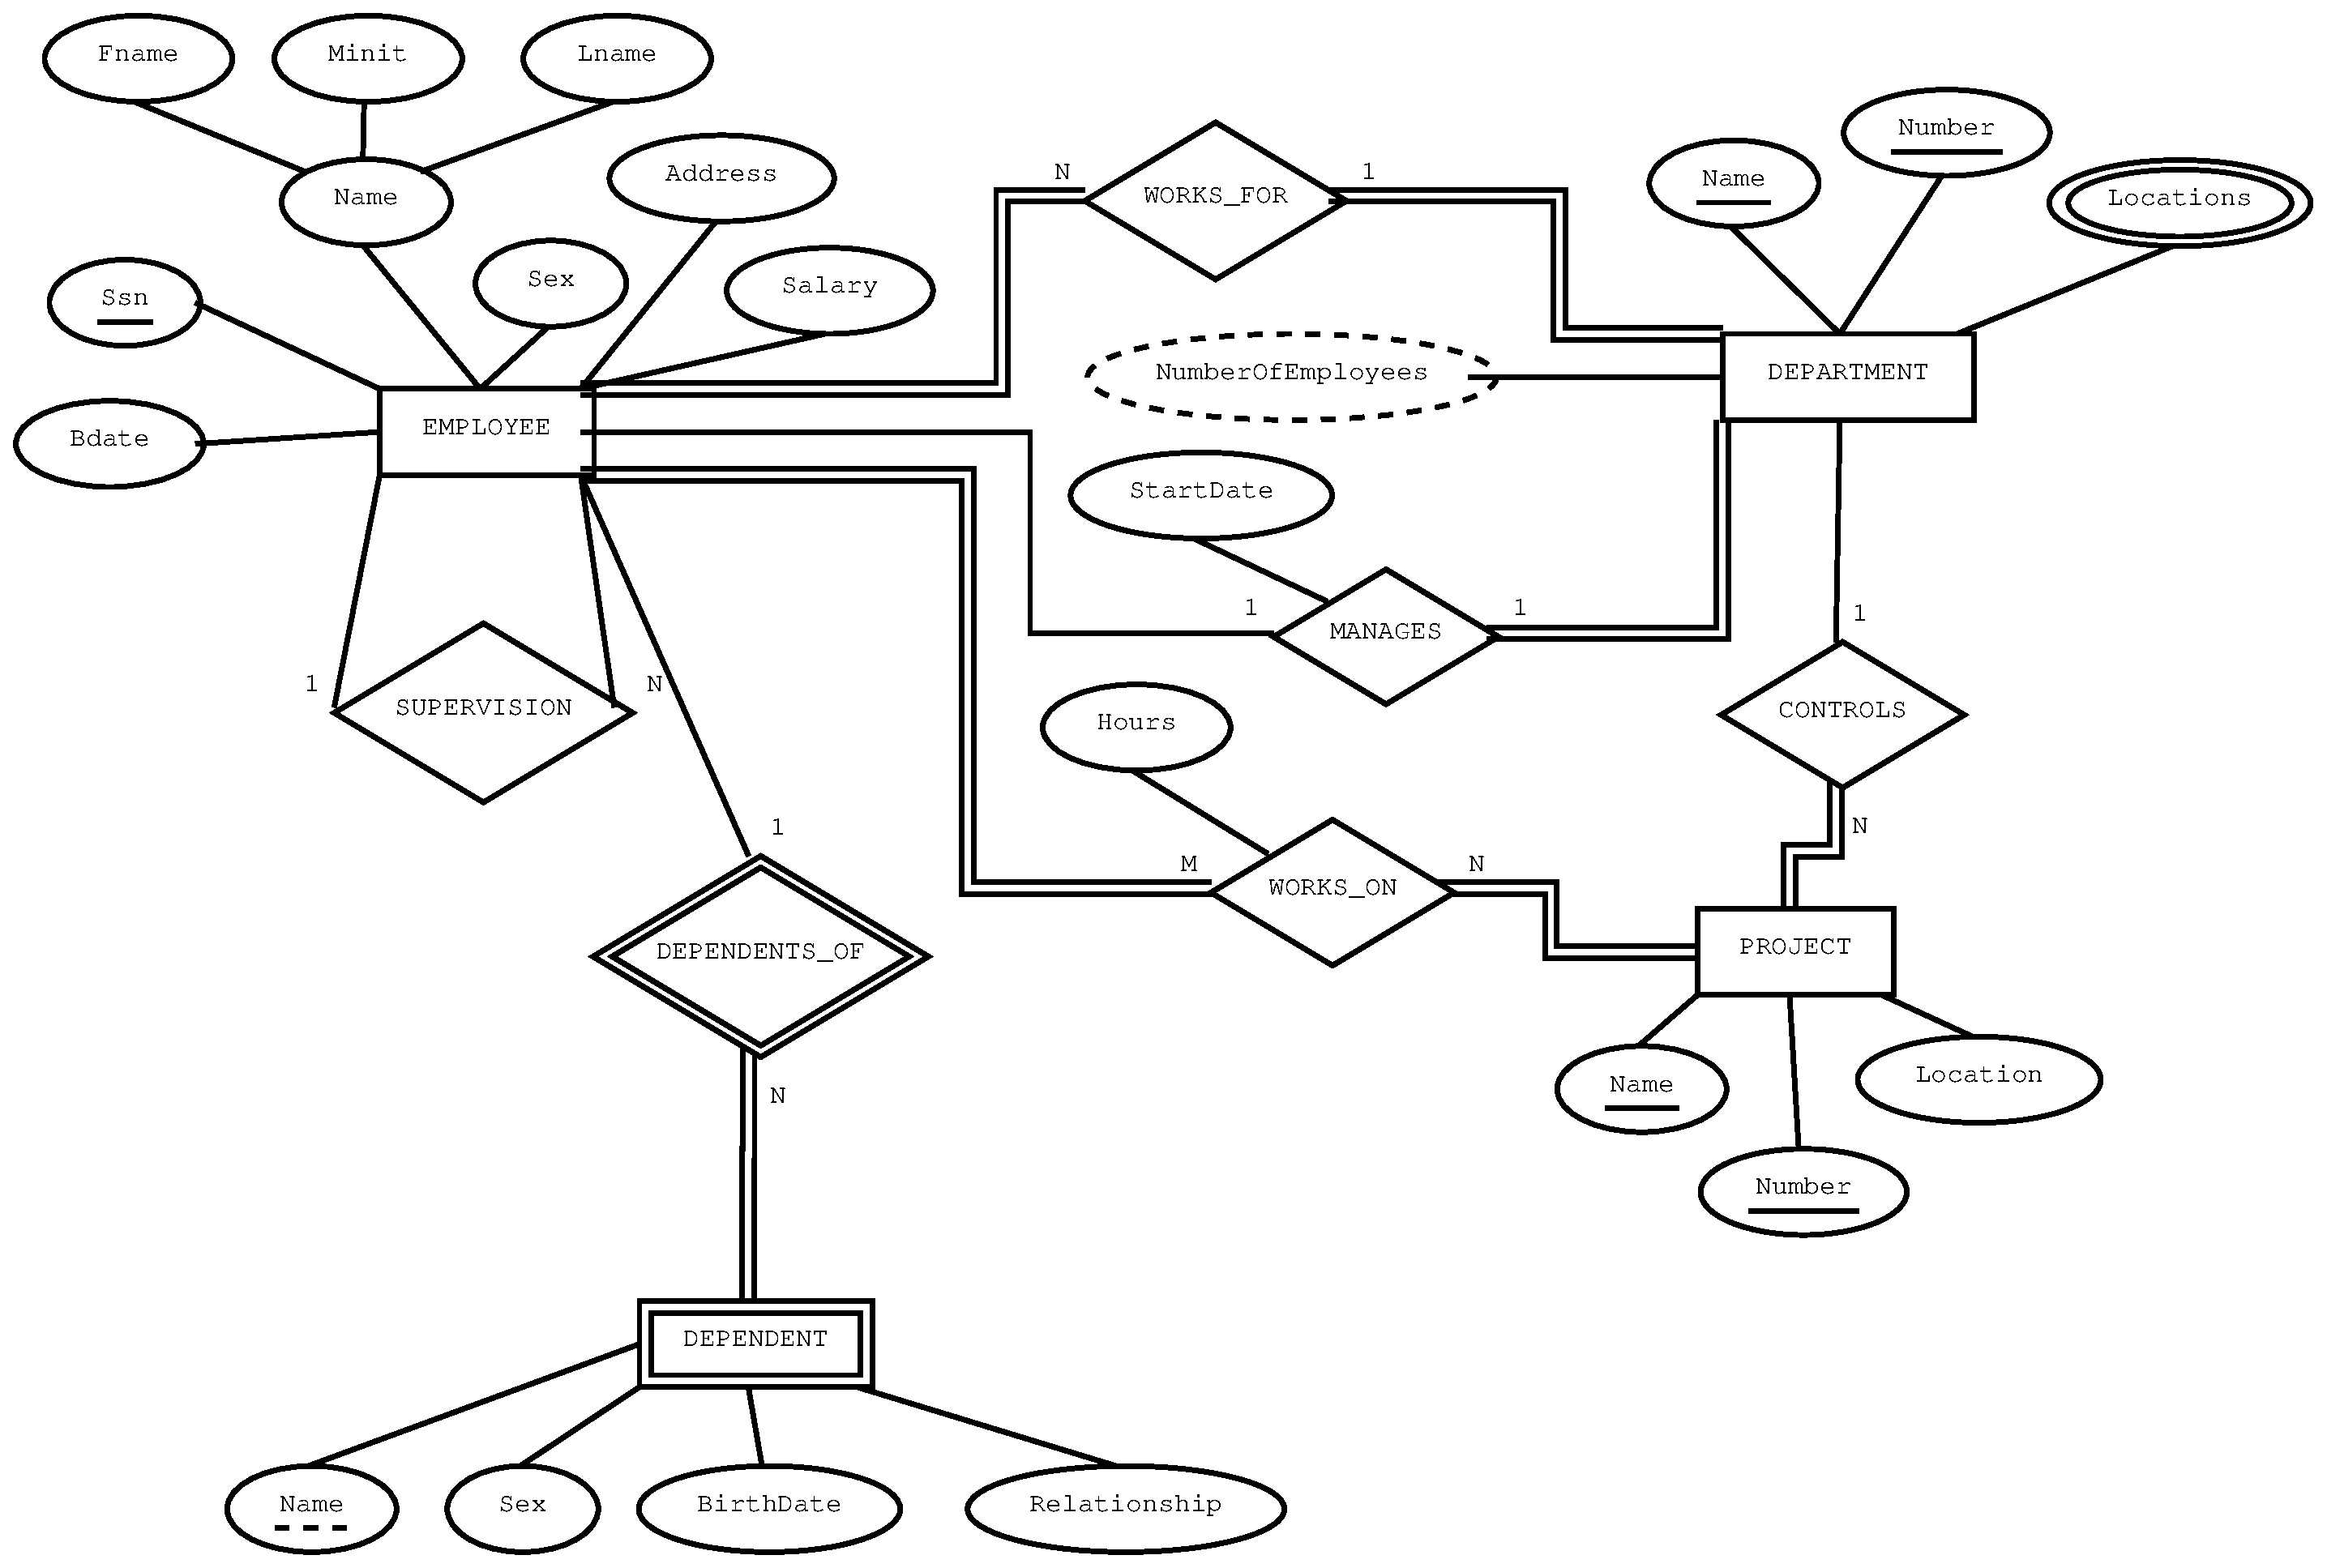
\includegraphics[width=0.6\textwidth]{exemplos/diagramas/ER.eps}
    \fonte{Indicar autor original.}
\end{figure}

\begin{figure}
    \centering
    \caption{Exemplo de diagrama - salvo imagem vetorizada - SVG}
    \label{fig:uml_dia_vetorizado_svg}
    \includesvg[inkscapelatex=false,width=0.6\textwidth]{exemplos/diagramas/ER.svg}
    \fonte{Indicar autor original.}
\end{figure}



% generated by Plantuml 7997beta
\definecolor{plantucolor0000}{RGB}{254,254,206}
\definecolor{plantucolor0001}{RGB}{168,0,54}
\definecolor{plantucolor0002}{RGB}{173,209,178}
\definecolor{plantucolor0003}{RGB}{0,0,0}
\definecolor{plantucolor0004}{RGB}{0,0,255}

\begin{figure}[htb]
    \centering
    \caption{\label{diagramauml}Exemplo de Diagrama UML gerado a partir do PlantUML}
\begin{tikzpicture}[yscale=-1]
\draw[color=plantucolor0001,fill=plantucolor0000,line width=1.5pt] (131pt,29pt) rectangle (223pt,90.8359pt);
\draw[color=plantucolor0001,fill=plantucolor0002,line width=1.0pt] (146pt,45pt) ellipse (11pt and 11pt);
\draw[color=black,fill=black] (148.7656pt,40.875pt) ..controls (148.9219pt,40.6563pt) .. (149.1094pt,40.5469pt) ..controls (149.2969pt,40.4375pt) .. (149.5156pt,40.4375pt) ..controls (149.8906pt,40.4375pt) .. (150.125pt,40.6953pt) ..controls (150.3594pt,40.9531pt) .. (150.3594pt,41.5625pt) -- (150.3594pt,43.0156pt) ..controls (150.3594pt,43.625pt) .. (150.125pt,43.8906pt) ..controls (149.8906pt,44.1563pt) .. (149.5156pt,44.1563pt) ..controls (149.1719pt,44.1563pt) .. (148.9688pt,43.9531pt) ..controls (148.7656pt,43.7656pt) .. (148.6563pt,43.25pt) ..controls (148.6094pt,42.8906pt) .. (148.4219pt,42.7031pt) ..controls (148.0938pt,42.3281pt) .. (147.4844pt,42.1094pt) ..controls (146.875pt,41.8906pt) .. (146.25pt,41.8906pt) ..controls (145.4844pt,41.8906pt) .. (144.8516pt,42.2188pt) ..controls (144.2188pt,42.5469pt) .. (143.7266pt,43.2969pt) ..controls (143.2344pt,44.0469pt) .. (143.2344pt,45.0781pt) -- (143.2344pt,46.1719pt) ..controls (143.2344pt,47.4063pt) .. (144.125pt,48.2266pt) ..controls (145.0156pt,49.0469pt) .. (146.6094pt,49.0469pt) ..controls (147.5469pt,49.0469pt) .. (148.2031pt,48.7969pt) ..controls (148.5938pt,48.6406pt) .. (149.0156pt,48.2031pt) ..controls (149.2813pt,47.9375pt) .. (149.4297pt,47.8594pt) ..controls (149.5781pt,47.7813pt) .. (149.7813pt,47.7813pt) ..controls (150.1094pt,47.7813pt) .. (150.3672pt,48.0391pt) ..controls (150.625pt,48.2969pt) .. (150.625pt,48.6406pt) ..controls (150.625pt,48.9844pt) .. (150.2813pt,49.3906pt) ..controls (149.7813pt,49.9688pt) .. (148.9844pt,50.2969pt) ..controls (147.9063pt,50.75pt) .. (146.6094pt,50.75pt) ..controls (145.0938pt,50.75pt) .. (143.8906pt,50.125pt) ..controls (142.9063pt,49.625pt) .. (142.2188pt,48.5547pt) ..controls (141.5313pt,47.4844pt) .. (141.5313pt,46.2031pt) -- (141.5313pt,45.0469pt) ..controls (141.5313pt,43.7188pt) .. (142.1484pt,42.5703pt) ..controls (142.7656pt,41.4219pt) .. (143.8594pt,40.8047pt) ..controls (144.9531pt,40.1875pt) .. (146.1875pt,40.1875pt) ..controls (146.9219pt,40.1875pt) .. (147.5703pt,40.3516pt) ..controls (148.2188pt,40.5156pt) .. (148.7656pt,40.875pt);
\node at (160pt,37.4531pt)[below right]{Subscriber};
\draw[color=plantucolor0001,line width=1.5pt] (132pt,61pt) -- (222pt,61pt);
\node at (137pt,65pt)[below right]{subscriberId};
\draw[color=plantucolor0001,line width=1.5pt] (132pt,82.8359pt) -- (222pt,82.8359pt);
\draw[color=plantucolor0001,fill=plantucolor0000,line width=1.5pt] (31pt,212pt) rectangle (137pt,273.8359pt);
\draw[color=plantucolor0001,fill=plantucolor0002,line width=1.0pt] (46pt,228pt) ellipse (11pt and 11pt);
\draw[color=black,fill=black] (48.7656pt,223.875pt) ..controls (48.9219pt,223.6563pt) .. (49.1094pt,223.5469pt) ..controls (49.2969pt,223.4375pt) .. (49.5156pt,223.4375pt) ..controls (49.8906pt,223.4375pt) .. (50.125pt,223.6953pt) ..controls (50.3594pt,223.9531pt) .. (50.3594pt,224.5625pt) -- (50.3594pt,226.0156pt) ..controls (50.3594pt,226.625pt) .. (50.125pt,226.8906pt) ..controls (49.8906pt,227.1563pt) .. (49.5156pt,227.1563pt) ..controls (49.1719pt,227.1563pt) .. (48.9688pt,226.9531pt) ..controls (48.7656pt,226.7656pt) .. (48.6563pt,226.25pt) ..controls (48.6094pt,225.8906pt) .. (48.4219pt,225.7031pt) ..controls (48.0938pt,225.3281pt) .. (47.4844pt,225.1094pt) ..controls (46.875pt,224.8906pt) .. (46.25pt,224.8906pt) ..controls (45.4844pt,224.8906pt) .. (44.8516pt,225.2188pt) ..controls (44.2188pt,225.5469pt) .. (43.7266pt,226.2969pt) ..controls (43.2344pt,227.0469pt) .. (43.2344pt,228.0781pt) -- (43.2344pt,229.1719pt) ..controls (43.2344pt,230.4063pt) .. (44.125pt,231.2266pt) ..controls (45.0156pt,232.0469pt) .. (46.6094pt,232.0469pt) ..controls (47.5469pt,232.0469pt) .. (48.2031pt,231.7969pt) ..controls (48.5938pt,231.6406pt) .. (49.0156pt,231.2031pt) ..controls (49.2813pt,230.9375pt) .. (49.4297pt,230.8594pt) ..controls (49.5781pt,230.7813pt) .. (49.7813pt,230.7813pt) ..controls (50.1094pt,230.7813pt) .. (50.3672pt,231.0391pt) ..controls (50.625pt,231.2969pt) .. (50.625pt,231.6406pt) ..controls (50.625pt,231.9844pt) .. (50.2813pt,232.3906pt) ..controls (49.7813pt,232.9688pt) .. (48.9844pt,233.2969pt) ..controls (47.9063pt,233.75pt) .. (46.6094pt,233.75pt) ..controls (45.0938pt,233.75pt) .. (43.8906pt,233.125pt) ..controls (42.9063pt,232.625pt) .. (42.2188pt,231.5547pt) ..controls (41.5313pt,230.4844pt) .. (41.5313pt,229.2031pt) -- (41.5313pt,228.0469pt) ..controls (41.5313pt,226.7188pt) .. (42.1484pt,225.5703pt) ..controls (42.7656pt,224.4219pt) .. (43.8594pt,223.8047pt) ..controls (44.9531pt,223.1875pt) .. (46.1875pt,223.1875pt) ..controls (46.9219pt,223.1875pt) .. (47.5703pt,223.3516pt) ..controls (48.2188pt,223.5156pt) .. (48.7656pt,223.875pt);
\node at (60pt,220.4531pt)[below right]{AccumUsage};
\draw[color=plantucolor0001,line width=1.5pt] (32pt,244pt) -- (136pt,244pt);
\node at (37pt,248pt)[below right]{subscriberId};
\draw[color=plantucolor0001,line width=1.5pt] (32pt,265.8359pt) -- (136pt,265.8359pt);
\draw[color=plantucolor0001,fill=plantucolor0000,line width=1.5pt] (221pt,191pt) rectangle (318pt,294.3438pt);
\draw[color=plantucolor0001,fill=plantucolor0002,line width=1.0pt] (240.05pt,207pt) ellipse (11pt and 11pt);
\draw[color=black,fill=black] (242.8156pt,202.875pt) ..controls (242.9719pt,202.6563pt) .. (243.1594pt,202.5469pt) ..controls (243.3469pt,202.4375pt) .. (243.5656pt,202.4375pt) ..controls (243.9406pt,202.4375pt) .. (244.175pt,202.6953pt) ..controls (244.4094pt,202.9531pt) .. (244.4094pt,203.5625pt) -- (244.4094pt,205.0156pt) ..controls (244.4094pt,205.625pt) .. (244.175pt,205.8906pt) ..controls (243.9406pt,206.1563pt) .. (243.5656pt,206.1563pt) ..controls (243.2219pt,206.1563pt) .. (243.0188pt,205.9531pt) ..controls (242.8156pt,205.7656pt) .. (242.7063pt,205.25pt) ..controls (242.6594pt,204.8906pt) .. (242.4719pt,204.7031pt) ..controls (242.1438pt,204.3281pt) .. (241.5344pt,204.1094pt) ..controls (240.925pt,203.8906pt) .. (240.3pt,203.8906pt) ..controls (239.5344pt,203.8906pt) .. (238.9016pt,204.2188pt) ..controls (238.2688pt,204.5469pt) .. (237.7766pt,205.2969pt) ..controls (237.2844pt,206.0469pt) .. (237.2844pt,207.0781pt) -- (237.2844pt,208.1719pt) ..controls (237.2844pt,209.4063pt) .. (238.175pt,210.2266pt) ..controls (239.0656pt,211.0469pt) .. (240.6594pt,211.0469pt) ..controls (241.5969pt,211.0469pt) .. (242.2531pt,210.7969pt) ..controls (242.6438pt,210.6406pt) .. (243.0656pt,210.2031pt) ..controls (243.3313pt,209.9375pt) .. (243.4797pt,209.8594pt) ..controls (243.6281pt,209.7813pt) .. (243.8313pt,209.7813pt) ..controls (244.1594pt,209.7813pt) .. (244.4172pt,210.0391pt) ..controls (244.675pt,210.2969pt) .. (244.675pt,210.6406pt) ..controls (244.675pt,210.9844pt) .. (244.3313pt,211.3906pt) ..controls (243.8313pt,211.9688pt) .. (243.0344pt,212.2969pt) ..controls (241.9563pt,212.75pt) .. (240.6594pt,212.75pt) ..controls (239.1438pt,212.75pt) .. (237.9406pt,212.125pt) ..controls (236.9563pt,211.625pt) .. (236.2688pt,210.5547pt) ..controls (235.5813pt,209.4844pt) .. (235.5813pt,208.2031pt) -- (235.5813pt,207.0469pt) ..controls (235.5813pt,205.7188pt) .. (236.1984pt,204.5703pt) ..controls (236.8156pt,203.4219pt) .. (237.9094pt,202.8047pt) ..controls (239.0031pt,202.1875pt) .. (240.2375pt,202.1875pt) ..controls (240.9719pt,202.1875pt) .. (241.6203pt,202.3516pt) ..controls (242.2688pt,202.5156pt) .. (242.8156pt,202.875pt);
\node at (254.95pt,199.4531pt)[below right]{IpSession};
\draw[color=plantucolor0001,line width=1.5pt] (222pt,223pt) -- (317pt,223pt);
\node at (227pt,227pt)[below right]{ipAddress};
\node at (227pt,240.8359pt)[below right]{specificData};
\node at (227pt,254.6719pt)[below right]{sapcOriginStateId};
\node at (227pt,268.5078pt)[below right]{apnId};
\draw[color=plantucolor0001,line width=1.5pt] (222pt,286.3438pt) -- (317pt,286.3438pt);
\draw[color=plantucolor0004] (191.942pt,90.081pt) ..controls (205.204pt,115.893pt) and (224.952pt,154.325pt) .. (241.265pt,186.076pt);
\draw[color=plantucolor0004,fill=plantucolor0004] (243.646pt,190.709pt) -- (243.0894pt,180.8759pt) -- (241.3604pt,186.262pt) -- (235.9742pt,184.5329pt) -- (243.646pt,190.709pt) -- cycle;
\node at (191.0584pt,98.9168pt)[below right]{1};
\node at (230.3817pt,166.6703pt)[below right]{1..*};
\draw[color=plantucolor0001] (162.058pt,90.081pt) ..controls (145.645pt,122.023pt) and (119.302pt,173.295pt) .. (101.824pt,207.31pt);
\draw[color=plantucolor0001,fill=plantucolor0001] (99.5252pt,211.784pt) -- (107.1969pt,205.6078pt) -- (101.8108pt,207.337pt) -- (100.0816pt,201.9509pt) -- (99.5252pt,211.784pt) -- cycle;
\node at (143.0082pt,98.7264pt)[below right]{1};
\node at (101.801pt,187.522pt)[below right]{0..1};
\end{tikzpicture}
	\legend{Fonte: Exemplos PlantUML.}
\end{figure}

A \autoref{fig_diag_virado} exemplifica como utilizar uma imagem em formato paisagem (página inteira). Obs: Utilizamos propositalmente uma imagem não vetorizada de forma a ilustrar o procedimento e também para apresentar que a qualidade não fica boa o suficiente para leitura. Uma versão vetorizada dessa figura teria qualidade melhor.


% observe que a imagem a seguir teve que ser ajustada para caber corretamente na página
% por não ser uma imagem vetorizada a qualidade não é a melhor possivel
\begin{sidewaysfigure}[htb]
    \centering
	\caption{\label{fig_diag_virado}Diagrama Virado - Exemplo}
	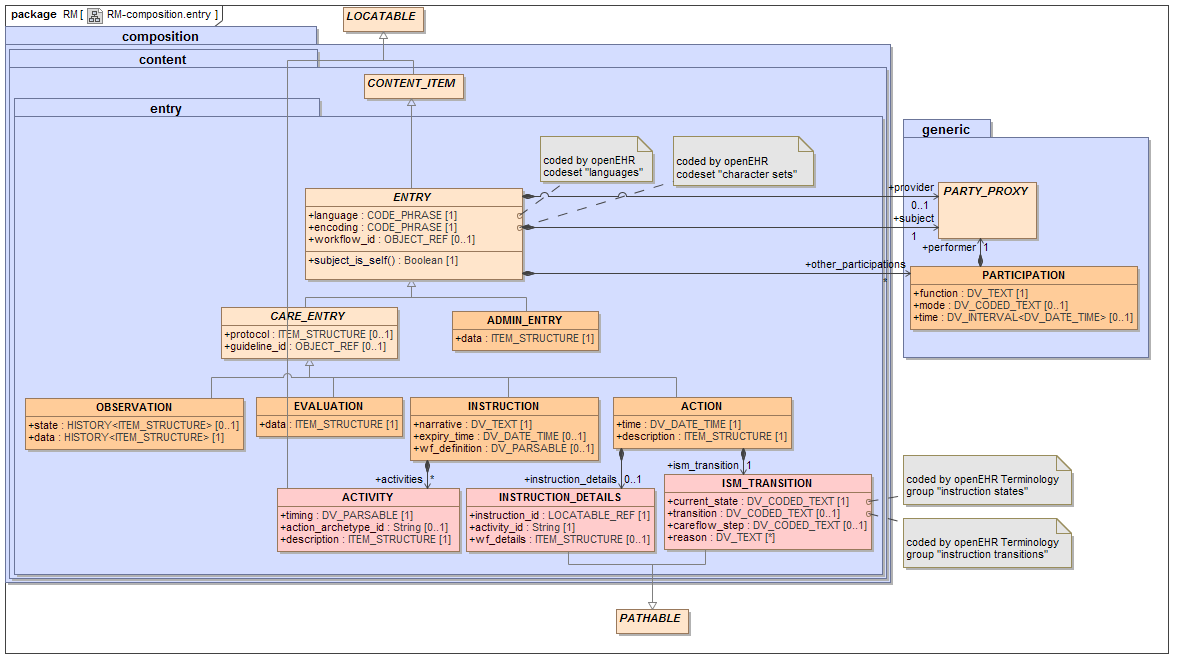
\includegraphics[width=0.9\textwidth]{exemplos/exemplo_diag_horizontal.png}
	\fonte{\citeonline{openehrCompositionEntry}.}
\end{sidewaysfigure}


\subsection{Impressão em folhas formato A3}

A página seguinte em A3 permite a impressão de diagramas grandes que não podem ser visualizados facilmente em folha padrão A4. Lembre que algumas impressoras podem ter problemas com isso, então selecione somente as páginas A4 ao imprimir e depois imprima separadamente a página A3.

A \autoref{fig_logo_A3} utiliza a mesma imagem da \autoref{fig_logo} e foi ampliada para demonstrar a essa possibilidade de impressão de grandes imagens em A3.

Observe que o código de exemplo vai gerar uma quebra de página no local onde for definida a página A3, por isso não deve ser utilizado entre textos para evitar grandes espaços em branco.

Folhas impressas em A3 ou tamanhos maiores devem ser dobradas seguindo o padrão definido pela \ac{abnt}. 


Cuidado ao utilizar folhas A3 em um documento impresso em frente e verso pois a numeração das páginas seguintes pode ser impressa de forma incorreta (posição do número na página). Uma alternativa para esta situação é manter todas páginas impressas em A3 no último apêndice, fazendo as referencias corretas durante o texto.



 \afterpage{%
 \begin{PAGINA-A3}

 \begin{figure}[p]
     \centering%
 	\caption{\label{fig_logo_A3}Logotipo \acs{ifsp} em página A3}
     \fcolorbox{red}{yellow}{ 
\includegraphics[height=\textheight,width=\textwidth,keepaspectratio]{\ifspprefixo/logo-02.jpg}}%
 	\legend{Com borda para demonstrar os limites}
   \fonte{citar o autor da Figura(xxx).}
 \end{figure}

 \end{PAGINA-A3}
 }





% ---
% Conclusão (outro exemplo de capítulo sem numeração e presente no sumário)
% Dependendo do trabalho desenvolvido ele pode ter uma Conclusão ou Considerações finais
% Para trabalhos de disciplina utilizar Considerações Finais
% ---
\chapter{Considerações Finais}
% Exemplo de como adicionar linha adicional no sumário
Com a matéria de Projeto Integrado I e II (PI1A5 e PI2A6), foi possível vivenciar, de fato, as etapas e desafios que envolvem desenvolver um software e sua documentação.

A experiência de realizar o projeto envolveu, acima de tudo, dificuldades diversas às quais foram necessárias adaptações, fossem elas individuais ou da equipe inteira. Todas essas dificuldades foram de extremo valor, já que puderam mostrar o quão importante são alguns fatores como: comunicação, sinceridade, atenção e proatividade.

Como maiores pontos de dificuldade pelos quais a equipe passou, pode-se citar o conhecimento sobre o tema escolhido, conhecimento técnico sobre as ferramentas de desenvolvimento, gestão de tempo e informações sobre as requisições de cada entrega e, por fim, a documentação LaTeX. Para todos esses pontos de falha foi crucial que houvessem reuniões, alinhamentos e divisão de tarefas balanceadamente, para que não houvesse prejuízo para nenhuma das partes.

Foi preciso esforço de todos os membros da equipe para se informarem acerca do tema escolhido, a neurodiversidade, para que, dessa forma, fossem evitados equívocos de terminologias utilizadas e falta de fontes de informação sobre como é a rotina das pessoas neurodiversas. Quanto aos outros pontos de dificuldade pontuados, foram realizadas diversas agendas e conversas informais para disseminação de conhecimento entre os membros, para que, o quanto antes, todos estivessem alinhados sobre todos os pontos do projeto.

Ao fim do projeto foi possível perceber a evolução de todos os envolvidos, tanto em âmbitos técnicos quanto em quesitos comportamentais, além de ser possível perceber o quão mais entrosada a equipe estava.



% ----------------------------------------------------------
% Finaliza a parte no bookmark do PDF
% para que se inicie o bookmark na raiz
% e adiciona espaço de parte no Sumário
% ----------------------------------------------------------
\phantompart

% ----------------------------------------------------------
% ELEMENTOS PÓS-TEXTUAIS
% ----------------------------------------------------------
\postextual
% ----------------------------------------------------------

% ----------------------------------------------------------
% Referências bibliográficas
% ----------------------------------------------------------
\bibliography{referencias,exemplos/abntex2-doc-abnt-6023}

% ----------------------------------------------------------
% Glossário
% ----------------------------------------------------------
%
%
\ifdef{\printnoidxglossary}{
    \addcontentsline{toc}{chapter}{GLOSSÁRIO}
    \printnoidxglossary[style=glossario]
    %\printglossaries
}{}

% ----------------------------------------------------------
% Apêndices
% Documentos gerados pelo próprio autor
% ----------------------------------------------------------

% ---
% Inicia os apêndices
% ---
\begin{apendicesenv}

% Imprime uma página indicando o início dos apêndices
\partapendices

	\chapter{Especificações de Casos de Uso}
	\label{casos-de-uso-especificacao}
	
	
	\begin{itemize}
		\item UC01: Fazer Login - Este uso de caso é abordado quando o cliente for fazer um cadastro na plataforma. O \autoref{casos-de-uso1} informa uma descrição, o fluxo básico de cadastro, um fluxo alternativo, pré-condições necessárias para conseguir fazer o uso de caso e pós-condições quando o uso de caso é concluído com sucesso.\\			
	\end{itemize}

\begin{quadro}[htb]
	\centering
	\ABNTEXfontereduzida
	\caption[Caso de Uso Fazer Login]{Caso de Uso Fazer Login}
	\label{casos-de-uso1}
\end{quadro}
\begin{longtable}{|p{3.3cm}|p{12.3cm}|}
	\hline
	\thead{} & \thead{Ator} \\
	\hline
	\endfirsthead
	%
	\multicolumn{2}{c}{\scriptsize Fonte: Equipe diversaGente (2022).}%
	{{\bfseries \autoref{casos-de-uso1} continued from previous page}} \\
	\endhead
	Descrição & Ao realizar o processo de login, o usuário terá acesso a todas as funcionalidades do aplicativo como consultar o feed de notícias, ter acesso ao fórum podendo criar subcategorias e post e compartilhar informações nos canais de texto, enviar mensagens privadas a outras pessoas que também estão logadas no app e avaliar locais a partir da sua vivência deste estabelecimento \\
	\hline
	Fluxo Básico  & 
	\begin{enumerate}
		\item O usuário entra no aplicativo e visualiza a tela de login;
		\item O usuário insere seu email e senha;
		\item Usuário entra no aplicativo;
		\item O caso de uso é encerrado. 
	\end{enumerate}\\
	\hline
	Fluxo Alternativo  & O usuário esqueceu a senha:
	\begin{enumerate}
		\item O usuário entra no aplicativo e visualiza a tela de login;
		\item O usuário insere seu email e senha;
		\item O sistema informa que a senha inserida está incorreta.
		\item O usuário clica em "Esqueci minha senha";
		\item O sistema envia um e-mail para o ator para trocar a senha;
		\item O usuário abre o e-mail e redefine sua senha;
		\item O fluxo principal é recomeçado.
		\item O caso de uso é encerrado.
	\end{enumerate} \\
	\hline
	Fluxo Alternativo  &  Preenchimento incorreto da senha:
	\begin{enumerate}
		\item O usuário entra no aplicativo e visualiza a tela de login;
		\item O usuário insere seu email e senha;
		\item O sistema informa que a senha inserida está incorreta.
		\item O sistema informa que a senha inserida está incorreta.
		\item O caso de uso é encerrado. 
	\end{enumerate}\\
	\hline
	Fluxo Alternativo & Primeiro Acesso
	\begin{enumerate}
		\item O usuário entra no aplicativo e visualiza a tela de login;
		\item O usuário clica em "cadastrar";
		\item O sistema apresenta a tela de boas vindas;
		\item O usuário clica em "Avançar"
		\item O usuário insere as informações necessárias para o cadastramento no aplicativo;
		\item O usuário recebe a mensagem de "Cadastro feito com sucesso";
		\item O fluxo principal é começado para o usuário;
		\item O caso de uso é encerrado.
	\end{enumerate} \\
	\hline
	Fluxo Alternativo & Login Social (Google):
	\begin{enumerate}
		\item O usuário entra no aplicativo e visualiza a tela de login;
		\item O usuário clica no botão de realizar o login social;
		\item O sistema direciona o usuário para link do login social;
		\item O usuário faz sua autenticação com o email social e senha;
		\item O usuário retorna para tela do aplicativo já sendo direcionado para o fluxo principal do app;
		\item O caso de uso é encerrado. 
	\end{enumerate} \\
	\hline
	Pré-condições & Ter acesso à internet, o aplicativo previamente instalado e uma conta Google.
	\hline
	Pós-condições & Acesso a homepage do aplicativo e de todas as funcionalidades existentes no sistema. \\
	\hline
\end{longtable}
\fonte{Equipe diversaGente (2022)}


%--------------------------------------------------------------

\begin{itemize}
	\item UC02: Efetuar Cadastro - Este uso de caso é abordado quando o cliente for fazer um cadastro na plataforma. O 	\autoref{casos-de-uso2} informa uma descrição, o fluxo básico de cadastro, um fluxo alternativo, pré-condições necessárias para conseguir fazer o uso de caso e pós-condições quando o uso de caso é concluído com sucesso. \\
\end{itemize}


\begin{quadro}[htb]
	\centering
	\ABNTEXfontereduzida
	\caption[Caso de Uso Efetuar Cadastro]{Caso de Uso Efetuar Cadastro}
	\label{casos-de-uso2}
\end{quadro}
\begin{longtable}{|p{3.3cm}|p{12.3cm}|}
	\hline
	\thead{} & \thead{Ator} \\
	\hline
		\endfirsthead
	%
	\multicolumn{2}{c}{\scriptsize Fonte: Equipe diversaGente (2022).}%
	{{ \autoref{casos-de-uso2} continued from previous page}} \\
	\endhead
	Descrição & Esse caso terá como funcionalidade o cadastrar novos usuários na aplicação.\\
	\hline
	Fluxo Básico  & 
	\begin{enumerate}
		\item O usuário entra no aplicativo e visualiza a tela de login;
		\item O usuário clica em "cadastrar";
		\item O sistema apresenta a tela de boas vindas;
		\item O usuário clica em "Avançar";
		\item O usuário clica em "Cadastrar no App";
		\item O usuário insere as informações necessárias para o cadastramento no aplicativo;
		\item É retornado ao usuário: "Cadastro realizado com sucesso";
		\item O fluxo principal é começado para o usuário;
		\item O caso de uso é encerrado.. 
	\end{enumerate}\\
	\hline
	Fluxo Alternativo  & Cadastro com a conta Google:
	\begin{enumerate}
		\item O usuário entra no aplicativo e visualiza a tela de login;
		\item O usuário clica em "cadastrar";
		\item O sistema apresenta a tela de boas vindas;
		\item O usuário clica em "Avançar";
		\item O usuário clica em "Cadastrar com o Google";
		\item O sistema irá direcioná-lo para sua conta google para permitir acesso;
		\item O usuário é retornado para o aplicativo e recebe a mensagem de "Cadastro feito com sucesso";
		\item  O fluxo principal é começado para o usuário;
		\item O caso de uso é encerrado.
	\end{enumerate}\\
	\hline
	Pré-condições & Ter acesso à internet e o aplicativo previamente instalado.\\
	\hline
	Pós-condições & O Visitante vai se tornar um novo usuário da aplicação.\\
	\hline
\end{longtable}
\fonte{Equipe diversaGente (2022)}

%--------------------------------------------------------------
	
	\begin{itemize}
		\item UC03: Editar perfil -  Este uso de caso é abordado quando o cliente for editar o seu perfil na plataforma.
		O \autoref{casos-de-uso3} informa uma descrição, o fluxo básico de cadastro, um fluxo alternativo, pré-
		condições necessárias para conseguir fazer o uso de caso e pós-condições quando o uso de
		caso é concluído com sucesso. \\
		
	\end{itemize}
	
	
	\begin{quadro}[htb]
		\centering
		\ABNTEXfontereduzida
		\caption[Caso de Uso Editar Perfil]{Caso de Uso Editar Perfil}
		\label{casos-de-uso3}
	\end{quadro}	
	\begin{longtable}{|p{3.3cm}|p{12.3cm}|}
		\hline
		\thead{} & \thead{Ator} \\
		\hline
		
		\endfirsthead
		%
		\multicolumn{2}{c}{\scriptsize Fonte: Equipe diversaGente (2022).}%
		{{ \autoref{casos-de-uso3} continued from previous page}} \\
		\endhead
		
		Descrição & Esse caso de uso ocorre quando o usuário logado no aplicativo deseja alterar suas informações de perfil.\\
		\hline
		Fluxo Básico  &
		\begin{enumerate}
			\item O usuário seleciona a seção "Perfil";
			\item O usuário seleciona "Editar Perfil";
			\item O sistema exibe os dados do perfil: nome, data de nascimento, e-mail, neuro diversidades que tem interesse, abertura de mensagens privadas;
			\item O usuário seleciona o(s) dado(s) que deseja editar;
			\item O usuário atualiza as suas informações e pressiona no botão "Salvar";
			\item O sistema valida os dados conforme requeridos e atualiza o perfil do assinante;
			\item O caso de uso é encerrado. 
		\end{enumerate}\\
		\hline
		Pré-condições & Ter acesso à internet e estar previamente logado no aplicativo.\\
		\hline
		Pós-condições & Ao final das alterações feitas pelo usuário, a seção perfil deve estar atualizada.\\
		\hline
	\end{longtable}
	\fonte{Equipe diversaGente (2022)}
	
	%--------------------------------------------------------------
	
	\begin{itemize}
		\item UC04: Consultar mensagens no Fórum - Este uso de caso é abordado quando o cliente for editar o seu perfil na plataforma.
		O \autoref{casos-de-uso4} informa uma descrição, o fluxo básico de cadastro, um fluxo alternativo, pré-
		condições necessárias para conseguir fazer o uso de caso e pós-condições quando o uso de
		caso é concluído com sucesso. \\
		
	\end{itemize}
	
	\begin{quadro}[htb]
		\centering
		\ABNTEXfontereduzida
		\caption[Caso de Uso Consultar mensagens do Fórum]{Caso de Uso Consultar mensagens do Fórum}
		\label{casos-de-uso4}
	\end{quadro}
	\begin{longtable}{|p{3.3cm}|p{12.3cm}|}
		\hline
		\thead{} & \thead{Ator} \\
		\hline
				
		\endfirsthead
		%
		\multicolumn{2}{c}{\scriptsize Fonte: Equipe diversaGente (2022).}%
		{{ \autoref{casos-de-uso4} continued from previous page}} \\
		\endhead
		
		Descrição & O cliente deve encontrar todas as mensagens ocorridas dentro das subcategorias.\\
		\hline
		Fluxo Básico  & 
		\begin{enumerate}
			\item O usuário seleciona a seção "Fórum";
			\item O usuário seleciona a categoria desejada;
			\item O sistema mostra todas as subcategorias relacionadas categoria escolhida pelo usuário;
			\item O usuário escolhe uma subcategoria;
			\item O sistema mostra todas as mensagens ocorridas nesse canal de texto até o momento. 
			\item O caso de uso é encerrado.
		\end{enumerate}\\
		\hline
		Pré-condições & Ter acesso à internet e estar previamente logado no aplicativo.\\
		\hline
		Pós-condições & Ao final da escolha da subcategoria, deverá mostrar todas as mensagens do canal de texto.\\
		\hline
	\end{longtable}
	\fonte{Equipe diversaGente (2022)}
	
%--------------------------------------------------------------
	
	\begin{itemize}
		\item UC05: Remover mensagens no Fórum -Este uso de caso é abordado quando o cliente remover mensagens no fórum. O 	\autoref{casos-de-uso5} informa uma descrição, o fluxo básico de cadastro, pré-condições necessárias para conseguir fazer o uso de caso e pós-condições quando o uso de caso é concluído com sucesso. \\
	\end{itemize}

	
	\begin{quadro}[htb]
		\centering
		\ABNTEXfontereduzida
		\caption[Caso de Uso Remover mensagens no Fórum]{Caso de Uso Remover mensagens no Fórum}
		\label{casos-de-uso5}
	\end{quadro}
	\begin{longtable}{|p{3.3cm}|p{12.3cm}|}
		\hline
		\thead{} & \thead{Ator} \\
		\hline
						
		\endfirsthead
		%
		\multicolumn{2}{c}{\scriptsize Fonte: Equipe diversaGente (2022).}%
		{{ \autoref{casos-de-uso5} continued from previous page}} \\
		\endhead
		
		Descrição & Ao criar uma subcategoria, o cliente poderá excluir sua própria mensagem dentro do canal de texto e poderá excluir as mensagens de outros dentro dessa subcategoria que ele criou. O Administrador terá permissão de excluir as mensagens das subcategorias, até mesmo do criador dela.\\
		\hline
		Fluxo Básico  & 
		Para o cliente:
		\begin{enumerate}
			\item O usuário seleciona a seção "Fórum";
			\item O usuário seleciona a categoria desejada;
			\item O sistema mostra todas as subcategorias relacionadas à categoria escolhida pelo usuário;
			\item O usuário escolhe uma subcategoria;
			\item O sistema mostra todas as mensagens ocorridas nesse canal de texto até o momento. 
			\item O usuário seleciona a mensagem que deseja excluir;
			\item O sistema atualiza o canal de texto retirando a mensagem excluída. 
			\item O  caso de uso é encerrado. 
		\end{enumerate}\\
		\hline
		Fluxo Básico  & 
		Para o Administrador:
		\begin{enumerate}
			\item O administrador seleciona a seção "Fórum";
			\item O administrador seleciona a categoria desejada;
			\item O administrador mostra todas as subcategorias relacionadas à categoria escolhida pelo usuário;
			\item O administrador escolhe uma subcategoria;
			\item O sistema mostra todas as mensagens ocorridas nesse canal de texto até o momento. 
			\item O administrador seleciona a mensagem que deseja excluir;
			\item O sistema atualiza o canal de texto retirando a mensagem excluída. 
			\item O caso de uso é encerrado. 
		\end{enumerate}\\
		\hline
		Pré-condições & Para o Cliente: 
		
		O cliente deve estar logado no app e ser o criador do subcategoria escolhida.\\
		\hline
		Pré-Condições & Para o Administrador:
		
		Deve-ser ter o permissionamento de acesso necessário.
		\hline
		Pós-condições & O sistema deve atualizar o canal de texto já retirando a mensagem de texto excluída.
		\hline
	\end{longtable}
	\fonte{Equipe diversaGente (2022)}
	
%--------------------------------------------------------------
	
	\begin{itemize}
		\item UC06: Curtir mensagens no Fórum. Este uso de caso é abordado quando o cliente for curtir uma mensagem do fórum. O 	\autoref{casos-de-uso6} informa uma descrição, fluxo básico, pré-condições e  pós-condições.\\
	\end{itemize}

	\begin{quadro}[htb]
		\centering
		\ABNTEXfontereduzida
		\caption[Caso de Uso Curtir mensagens no Fórum]{Caso de Uso Curtir mensagens no Fórum}
		\label{casos-de-uso6}
	\end{quadro}

\pagebreak

		\begin{longtable}{|p{3.3cm}|p{12.3cm}|}
		\hline
		\thead{} & \thead{Ator} \\
		\hline
		Descrição & O usuário poderá curtir uma mensagem de texto dentro das subcategorias.\\
		\hline
						
		\endfirsthead
		%
		\multicolumn{2}{c}{\scriptsize Fonte: Equipe diversaGente (2022).}%
		{{ \autoref{casos-de-uso6} continued from previous page}} \\
		\endhead
		
		Fluxo Básico  & 
		\begin{enumerate}
			\item O usuário seleciona a seção "Fórum";
			\item O usuário seleciona a categoria desejada;
			\item O sistema mostra todas as subcategorias relacionadas categoria escolhida pelo usuário;
			\item O usuário escolhe uma subcategoria;
			\item O sistema mostra todas as mensagens ocorridas nesse canal de texto até o momento. 
			\item  O usuário seleciona a mensagem desejada e clica em "curtir mensagem";
			\item  O sistema atualiza o canal de texto;
			\item  O caso de uso é encerrado;
		\end{enumerate}\\
		\hline
		Pré-condições & Ter acesso à internet e estar previamente logado no aplicativo.\\
		\hline
		Pós-condições & O sistema irá atualizar o número de curtidas da mensagem selecionada pelo usuário.\\
		\hline
	
	\end{longtable}
	\fonte{Equipe diversaGente (2022)}
	
	\pagebreak

%--------------------------------------------------------------
	
	\begin{itemize}
		\item UC07: Criar categoria - Este uso de caso é abordado quando o cliente for curtir uma mensagem do fórum. O 	\autoref{casos-de-uso7}	informa uma descrição, o fluxo básico de cadastro, pré-condições necessárias para conseguir fazer o uso de caso e pós-condições quando o uso de caso é concluído com sucesso.\\
	\end{itemize}
	
	\begin{quadro}[htb]
		\centering
		\ABNTEXfontereduzida
		\caption[Caso de Uso Criar categoria]{Caso de Uso Criar categoria}
		\label{casos-de-uso7}
	\end{quadro}

	\begin{longtable}{|p{3.3cm}|p{12.3cm}|}
		\hline
		\thead{} & \thead{Ator} \\
		\hline
								
		\endfirsthead
		%
		\multicolumn{2}{c}{\scriptsize Fonte: Equipe diversaGente (2022).}%
		{{ \autoref{casos-de-uso7} continued from previous page}} \\
		\endhead
		
		Descrição & O Administrador tem permissão de criar uma categoria dentro do fórum.\\
		\hline
		Fluxo Básico  & 
		\begin{enumerate}
			\item O administrador seleciona a seção "Fórum";
			\item O administrador seleciona o botão "+";
			\item O sistema irá apresentar a opção "Criar uma Categoria";
			\item Ao clicar em criar uma categoria, o administrador deverá escrever o nome da categoria e clicar em "Criar canal de texto";
			\item O sistema atualizará com a nova categoria criada. 
			\item O caso de uso é encerrado. 
		\end{enumerate}\\
		\hline
		Pré-condições &O administrador deve ter a chave de permissão.
		\hline
		Pós-condições & O sistema mostrará a nova categoria criada pelo administrador e deve permitir que a partir dessa categoria sejam criadas subcategorias pelos usuários e administradores.\\
		\hline
	\end{longtable}
	\fonte{Equipe diversaGente (2022)}
		
%--------------------------------------------------------------
	
	\begin{itemize}
		\item UC08: Criar uma subcategoria - Este uso de caso é abordado quando o cliente for criar uma subcategoria. O \autoref{casos-de-uso8}	informa uma descrição, o fluxo básico de cadastro, pré-condições necessárias para conseguir fazer o uso de caso e pós-condições quando o uso de caso é concluído com sucesso.\\
	\end{itemize}

\pagebreak
	
	\begin{quadro}[htb]
		\centering
		\ABNTEXfontereduzida
		\caption[Caso de Uso Criar uma subcategoria]{Caso de Uso Criar uma subcategoria}
		\label{casos-de-uso8}
	\end{quadro}
	\begin{longtable}{|p{3.3cm}|p{12.3cm}|}
		\hline
		\thead{} & \thead{Ator} \\
		\hline
									
		\endfirsthead
		%
		\multicolumn{2}{c}{\scriptsize Fonte: Equipe diversaGente (2022).}%
		{{ \autoref{casos-de-uso8} continued from previous page}} \\
		\endhead
		
		Descrição & O cliente e/ou administrador devem conseguir criar subcategorias a partir das categorias já criadas pelo administrador.\\
		\hline
		Fluxo Básico  & 
		\begin{enumerate}
			\item O usuário seleciona a seção "Fórum";
			\item O usuário seleciona a categoria desejada;
			\item O usuário clica no botão "+" ao lado do nome da categoria selecionada;
			\item O usuário escreve o nome da subcategoria e clica em "Salvar"
			\item O sistema atualiza com a nova subcategoria criada. 
			\item O caso de uso é encerrado. 
		\end{enumerate}
		\hline
		Pré-condições & O cliente deve estar logado no app e o administrador deve ter a chave de permissão;
		\hline
		Pós-condições & O sistema mostrará a nova categoria criada pelo administrador ou usuário.\\
		\hline
	\end{longtable}
	\fonte{Equipe diversaGente (2022)}
	
%---------------------------------------------------------------
	
	\begin{itemize}
		\item UC09: Remover uma subcategoria - Este uso de caso é abordado quando o cliente for remover uma subcategoria. O 	\autoref{casos-de-uso9}	informa uma descrição, o fluxo básico de cadastro, pré-condições necessárias para conseguir fazer o uso de caso e pós-condições quando o uso de caso é concluído com sucesso.\\
	\end{itemize}
	
	\begin{quadro}[htb]
		\centering
		\ABNTEXfontereduzida
		\caption[Caso de Uso Remover uma subcategoria]{Caso de Uso Remover uma subcategoria}
		\label{casos-de-uso9}
	\end{quadro}
	
	\begin{longtable}{|p{3.3cm}|p{12.3cm}|}
		\hline
		\thead{} & \thead{Ator} \\
		\hline
							
		\endfirsthead
		%
		\multicolumn{2}{c}{\scriptsize Fonte: Equipe diversaGente (2022).}%
		{{ \autoref{casos-de-uso9} continued from previous page}} \\
		\endhead
		Descrição & O cliente e/ou administrador devem conseguir remover uma subcategoria. \\
		\hline
		Fluxo Básico  & Para o cliente
		\begin{enumerate}
			\item O usuário seleciona a seção "Fórum";
			\item O usuário seleciona uma categoria;
			\item O sistema mostra todas as subcategoria existentes;
			\item O cliente seleciona a subcategoria desejada;
			\item O cliente pressiona a subcategoria;
			\item Caso o cliente seja o criador dessa subcategoria, o sistema irá mostrar uma pop-up perguntando para o usuário se ele deseja excluir a subcategoria criada. 
			\item O usuário clica em "Sim";
			\item O sistema exclui a subcategoria;
			\item O caso de uso é encerrado. 
		\end{enumerate}
		\hline
		Fluxo Básico  & Para o administrador
		\begin{enumerate}
			\item O administrador seleciona a seção "Fórum";
			\item O administrador seleciona uma categoria;
			\item O sistema mostra todas as subcategoria existentes;
			\item O administrador seleciona a subcategoria desejada;
			\item O administrador pressiona a subcategoria;
			\item O sistema irá mostrar uma pop-up perguntando para o administrador se ele deseja excluir a subcategoria pressionada;
			\item O administrador clica em "Sim";
			\item O sistema exclui a subcategoria;
			\item O caso de uso é encerrado. 
		\end{enumerate}\\
		\hline
		Pré-condições & Para o cliente:
		
		O cliente deve estar logado no app e ser o criador do subcategoria escolhida. \\
		\hline
		Pré-condições & Para o administrador:
		
		Deve-ser ter o permissionamento de acesso necessário.
		\hline
		Pós-condições & O sistema irá atualizar removendo a subcategoria selecionada.\\
		\hline
	\end{longtable}
	\fonte{Equipe diversaGente (2022)}
	
	%-----------------------------------------------------------
	
	\begin{itemize}
		\item UC10: Criação do Local Avaliado - Este uso de caso é abordado quando o cliente for criar um local para ser avaliado. O \autoref{casos-de-uso10} informa uma descrição, o fluxo básico de cadastro, um fluxo de exceção, pré-condições necessárias para conseguir fazer o uso de caso e pós-condições quando o uso de caso é concluído com sucesso.\\	
	\end{itemize}
		
	\begin{quadro}[htb]
		\centering
		\ABNTEXfontereduzida
		\caption[Caso de Uso Criação do Local Avaliado]{Caso de Uso Criação do Local Avaliado}
		\label{casos-de-uso10}
	\end{quadro}
	\begin{longtable}{|p{3.3cm}|p{12.3cm}|}
		\hline
		\thead{} & \thead{Ator} \\
		\hline
		
										
		\endfirsthead
		%
		\multicolumn{2}{c}{\scriptsize Fonte: Equipe diversaGente (2022).}%
		{{ \autoref{casos-de-uso10} continued from previous page}} \\
		\endhead
		
		Descrição & O usuário poderá avaliar positivamente ou negativamente os estabelecimentos que ele queira recomendar para outras pessoas dentro da rede social.\\
		\hline
		Fluxo Básico  & 
		\begin{enumerate}
			\item O usuário clica na seção 'Locais Avaliados';
			\item O usuário clica na aba 'Meus Locais Avaliados';
			\item O usuário clica em "Adicionar Avaliação";
			\item O sistema fornece a parte de "Adicionar Avaliação";
			\item O usuário cadastra a avaliação e clica em "Salvar";
			\item O sistema busca identificar e confirmar os dados inseridos pelo usuário.
			\item O sistema retorna "Avaliação Adicionada" e adiciona na lista de locais avaliados;
			\item O caso de uso é encerrado.
		\end{enumerate}
		\hline
		Fluxo de Exceção & O usuário não insere todos os dados necessários: 
		\begin{enumerate}
			\item O usuário clica na aba 'Meus Locais Avaliados';
			\item O usuário clica em "Adicionar Avaliação";
			\item O sistema fornece a parte de "Adicionar Avaliação";
			\item O usuário cadastra a avaliação e clica em "Salvar";
			\item O sistema retorna os dados obrigatórios que o usuário não inseriu ao cadastrar e impede que a avaliação seja salva;
			\item O caso de uso é encerrado. 
		\end{enumerate}
		\hline
		Pré-condições & Ter acesso à internet e estar previamente logado no aplicativo.
		\hline
		Pós-condições & Apresentar o Local Avaliado cadastrado pelo usuário na aba ’Locais Avaliados’.
		\hline
	\end{longtable}
	\fonte{Equipe diversaGente (2022)}
	\pagebreak
	
%---------------------------------------------------------------
	
	\begin{itemize}
		\item UC11: Consultar Locais Avaliados - Este uso de caso é abordado quando o cliente for consultar locais avaliados. O \autoref{casos-de-uso11} informa uma descrição, o fluxo básico de cadastro, pré-condições necessárias para conseguir fazer o uso de caso e pós-condições quando o uso de caso é concluído com sucesso.	
	\end{itemize}
	
	\begin{quadro}[htb]
		\centering
		\ABNTEXfontereduzida
		\caption[Caso de Uso Consultar Locais Avaliados]{Consultar Locais Avaliados}
		\label{casos-de-uso11}
	\end{quadro}
	\begin{longtable}{|p{3.3cm}|p{12.3cm}|}
		\hline
		\thead{} & \thead{Ator} \\
		\hline
										
		\endfirsthead
		%
		\multicolumn{2}{c}{\scriptsize Fonte: Equipe diversaGente (2022).}%
		{{ \autoref{casos-de-uso11} continued from previous page}} \\
		\endhead
		
		Descrição & Consultar todos os locais avaliados já adicionados pelos usuários.\\
		\hline
		Fluxo Básico  & 
		\begin{enumerate}
			\item O usuário clica na seção 'Locais Avaliados';
			\item O usuário clica na aba 'Todos Locais Avaliados';  
			\item O usuário clica no nome de um local avaliado;
			\item O usuário visualiza a avaliação;
			\item O caso de uso é encerrado. 
		\end{enumerate}\\
		\hline
		Pré-condições & Ter acesso à internet e estar previamente logado no aplicativo.
		\hline
		Pós-condições & Apresentar todos os locais avaliados cadastrados e seus respectivos dados.\\
		\hline
	\end{longtable}
	\fonte{Equipe diversaGente (2022)}
	
	%---------------------------------------------------------------
	
	\begin{itemize}
		\item UC12: Editar Locais Avaliados - Este uso de caso é abordado quando o cliente for editar um local avaliado. O 	\autoref{casos-de-uso12} informa uma descrição, o fluxo básico de cadastro, pré-condições necessárias para conseguir fazer o uso de caso e pós-condições quando o uso de caso é concluído com sucesso.\\
	\end{itemize}
		
	\begin{quadro}[htb]
		\centering
		\ABNTEXfontereduzida
		\caption[Caso de Uso Editar Locais Avaliados]{Caso de Uso Editar Locais Avaliados}
		\label{casos-de-uso12}
	\end{quadro}
	\begin{longtable}{|p{3.3cm}|p{12.3cm}|}
		\hline
		\thead{} & \thead{Ator} \\
		\hline
		
										
		\endfirsthead
		%
		\multicolumn{2}{c}{\scriptsize Fonte: Equipe diversaGente (2022).}%
		{{ \autoref{casos-de-uso12} continued from previous page}} \\
		\endhead
		
		Descrição & O usuário poderá editar as informações inseridas por ele na aba de 'Meus Locais Avaliados'.\\
		\hline
		Fluxo Básico  &
		\begin{enumerate}
			\item O usuário clica na aba 'Meus Locais Avaliados';
			\item O usuário pressiona o local avaliado na qual ele quer editar;
			\item O sistema mostra uma pop-up com a opção "Editar Local Avaliado";
			\item O usuário clica em "Editar Local Avaliado";
			\item O usuário edita as informações e clica em "Salvar";
			\item O sistema confirmar os dados inseridos pelo usuário;
			\item O caso de uso é encerrado. 
		\end{enumerate}
		\hline
		Pré-condições & Ter acesso à internet, estar logado no aplicativo e ser o criador do local avaliado em questão.
		\hline
		Pós-condições & O sistema deve apresentar o local avaliado com as novas informações inseridas pelo usuário.
		\hline
	\end{longtable}
	\fonte{Equipe diversaGente (2022)}
	%---------------------------------------------------------------
	
	
		\begin{itemize}
		\item UC13: Remover Local Avaliado - Este uso de caso é abordado quando o cliente remover um local avaliado. O \autoref{casos-de-uso13} informa uma descrição, o fluxo básico de cadastro, pré-condições necessárias para conseguir fazer o uso de caso e pós-condições quando o uso de caso é concluído com sucesso.\\		
	\end{itemize}
	
	\begin{quadro}[htb]
		\centering
		\ABNTEXfontereduzida
		\caption[Caso de Uso Remover Local Avaliado]{Caso de Uso Remover Local Avaliado}
		\label{casos-de-uso13}
	\end{quadro}
	\begin{longtable}{|p{3.3cm}|p{12.3cm}|}
		\hline
		\thead{} & \thead{Ator} \\
		\hline
										
		\endfirsthead
		%
		\multicolumn{2}{c}{\scriptsize Fonte: Equipe diversaGente (2022).}%
		{{ \autoref{casos-de-uso13} continued from previous page}} \\
		\endhead
		
		Descrição &O usuário poderá excluir o local avaliado inserido por ele na aba de 'Meus Locais Avaliados'.\\
		\hline
		Fluxo Básico  & 
		\begin{enumerate}
			\item O usuário clica na seção 'Locais Avaliados';
			\item O usuário clica na aba 'Meus Locais Avaliados';
			\item O usuário pressiona o local avaliado na qual ele quer excluir;
			\item O sistema mostra uma pop-up com a opção "Excluir Local Avaliado"; 
			\item O usuário clica em "Excluir Local Avaliado";
			\item O usuário exclui local avaliado";
			\item O sistema atualiza e retorna com a mensagem "local excluído com sucesso";
			\item O caso de uso é encerrado. 
		\end{enumerate}\\
		\hline
		Pré-condições & Ter acesso à internet, estar previamente logado no aplicativo e ser o criador da avaliação de local em questão.
		\hline
		Pós-condições & O sistema deve excluir o local avaliado escolhido pelo usuário da lista "Meus Locais Avaliados" e "Locais Avalaidos".\\
		\hline
	\end{longtable}
	\fonte{Equipe diversaGente (2022)}
	
	%---------------------------------------------------------------
	
	\begin{itemize}
		\item UC14: Visualizar Perfil dos usuários - Este uso de caso é abordado quando o cliente for visualizar um perfil de um outro usuário na plataforma. O \autoref{casos-de-uso14} informa uma descrição, o fluxo básico de cadastro, um fluxo alternativo, pré-condições necessárias para conseguir fazer o uso de caso e pós-condições quando o uso de caso é concluído com sucesso.\\	
	\end{itemize}
	
	\pagebreak
	
	\begin{quadro}[htb]
		\centering
		\ABNTEXfontereduzida
		\caption[Caso de Uso Visualizar Perfil dos usuários]{Caso de Uso Visualizar Perfil dos usuários}
		\label{casos-de-uso14}
	\end{quadro}
	\begin{longtable}{|p{3.3cm}|p{12.3cm}|}
		\hline
		\thead{} & \thead{Ator} \\
		\hline
										
		\endfirsthead
		%
		\multicolumn{2}{c}{\scriptsize Fonte: Equipe diversaGente (2022).}%
		{{ \autoref{casos-de-uso14} continued from previous page}} \\
		\endhead
		
		Descrição & Visualiza perfil do cliente quando clica na foto de perfil ou no nome do usuário.\\
		\hline
		Fluxo Básico  & 
		\begin{enumerate}
			\item O usuário clica na imagem do usuário;
			\item O usuário visualiza o perfil de outro usuário;
			\item O caso de uso está encerrado.
		\end{enumerate}\\
		\hline
		Fluxo Alternativo & 
		\begin{enumerate}
			\item O usuário clica no nome do usuário;
			\item O usuário visualiza o perfil de outro usuário;
			\item O caso de uso está encerrado.
		\end{enumerate}\\
		\hline
		Pré-condições & Ter acesso à internet e estar logado previamente no aplicativo.\\
		\hline
		Pós-condições & O sistema irá mostrar uma nova tela com todas as informações do usuário escolhido.\\
		\hline
	\end{longtable}
	\fonte{Equipe diversaGente (2022)}
	
	%---------------------------------------------------------------
	
	\begin{itemize}
		\item UC15: Troca de mensagens de texto em chat individual - Este uso de caso é abordado quando o cliente for trocar uma mensagem de texto com outro perfil. O \autoref{casos-de-uso15} informa uma descrição, o fluxo básico de ação, um fluxo alternativo, pré-condições necessárias para conseguir fazer o uso de caso e pós-condições quando o uso de caso é concluído com sucesso.\\
	\end{itemize}
	
	\begin{quadro}[htb]
		\centering
		\ABNTEXfontereduzida
		\caption[Caso de Uso Troca de mensagens de texto em chat individual]{Caso de Uso Troca de mensagens de texto em chat individual}
		\label{casos-de-uso15}
	\end{quadro}
	
	\begin{longtable}{|p{3.3cm}|p{12.3cm}|}
		\hline
		\thead{} & \thead{Ator} \\
		\hline
		
										
		\endfirsthead
		%
		\multicolumn{2}{c}{\scriptsize Fonte: Equipe diversaGente (2022).}%
		{{ \autoref{casos-de-uso15} continued from previous page}} \\
		\endhead
		
		Descrição &Nesse caso de uso, o usuário poderá enviar e receber mensagens por meio de um chat privado entre os usuários.\\
		\hline
		Fluxo Básico  & 
		\begin{enumerate}
			\item O usuário clica na aba "Chat";
			\item O usuário clica em um dos usuários que estão em sua lista;
			\item O usuário envia mensagem;
			\item O caso de uso é encerrado. 
		\end{enumerate}\\
		\hline
		Fluxo Alternativo & 
		Primeira vez do usuário enviando mensagem. 
		\begin{enumerate}
			\item O usuário clica na imagem ou no nome do outro usuário;
			\item O usuário visualiza o perfil desse usuário;
			\item O usuário clica em "Enviar Mensagem";
			\item O sistema abre o chat entre esses dois usuários;
			\item O usuário envia a mensagem;
			\item O caso de uso é encerrado 
		\end{enumerate}\\
		\hline
		Pré-condições & Ter acesso à internet e estar previamente logado no aplicativo\\
		\hline
		Pós-condições & O usuário deve ter sua mensagem entregue e recebida pelo outro usuário.\\
		\hline
	\end{longtable}
	\fonte{Equipe diversaGente (2022)}
	
	%---------------------------------------------------------------
	
	\begin{itemize}
		\item UC16: Visualizar notícias -Este uso de caso é abordado quando o cliente quiser visualizar uma notícia dentro da plataforma. O \autoref{casos-de-uso16} informa uma descrição, o fluxo básico de ação, pré-condições necessárias para a realização do caso e pós-condições da ação.\\
	\end{itemize}
	
	\begin{quadro}[htb]
		\centering
		\ABNTEXfontereduzida
		\caption[Caso de Uso Visualizar notícias]{Caso de Uso Visualizar notícias}
		\label{casos-de-uso16}
	\end{quadro}
	\begin{longtable}{|p{3.3cm}|p{12.3cm}|}
		\hline
		\thead{} & \thead{Ator} \\
		\hline
		
										
		\endfirsthead
		%
		\multicolumn{2}{c}{\scriptsize Fonte: Equipe diversaGente (2022).}%
		{{ \autoref{casos-de-uso16} continued from previous page}} \\
		\endhead
		
		Descrição & O usuário deverá visualizar todas as notícias dentro da seção "Feed de notícias".\\
		\hline
		Fluxo Básico  & 
		\begin{enumerate}
			\item O usuário logado entra na seção "Feed de notícias";
			\item O usuário visualiza as notícias;
			\item O caso de uso é encerrado. 
		\end{enumerate}\\
		\hline
		Fluxo Alternativo &
		\begin{enumerate}
			\item O usuário logado entra na seção "Feed de notícias";
			\item O usuário visualiza as notícias;
			\item O usuário clica em uma notícia;
			\item O sistema leva o usuário para uma nova tela com os detalhamentos da notícia clicada pelo usuário;
			\item O caso de uso é encerrado. 
		\end{enumerate}\\
		\hline
		Pré-condições & Ter acesso à internet e estar previamente logado no aplicativo.\\
		\hline
		Pós-condições & O sistema deve mostrar as notícias relacionadas ao tema de crianças neuro diversas.\\
		\hline
	\end{longtable}
	\fonte{Equipe diversaGente (2022)}
	
	%---------------------------------------------------------------
	
	\begin{itemize}
		\item UC17: Criar um Post -Este uso de caso é abordado quando o cliente quiser criar uma postagem na plataforma. O 	\autoref{casos-de-uso17} informa uma descrição, o fluxo básico de ação, pré-condições necessárias para a realização do caso e pós-condições da ação.\\
	\end{itemize}
	
	\begin{quadro}[htb]
		\centering
		\ABNTEXfontereduzida
		\caption[Caso de Uso Criar um Post]{Caso de Uso Criar um Post}
		\label{casos-de-uso17}
	\end{quadro}
	\begin{longtable}{|p{3.3cm}|p{12.3cm}|}
		\hline
		\thead{} & \thead{Ator} \\
		\hline
		
										
		\endfirsthead
		%
		\multicolumn{2}{c}{\scriptsize Fonte: Equipe diversaGente (2022).}%
		{{ \autoref{casos-de-uso17} continued from previous page}} \\
		\endhead
		
		Descrição & O usuário poderá criar um post a partir das subcategorias existentes. \\
		\hline
		Fluxo Básico  & 
		\begin{enumerate}
			\item O usuário seleciona uma subcategoria selecionada;
			\item O usuário clica no botão "+" ao lado do nome da subcategoria selecionada para criar o post;
			\item O usuário insere as informações necessárias para a criação do post;
			\item O usuário clica em "Criar Post"; 
			\item O caso de uso é encerrado. 
		\end{enumerate}\\
		\hline
		Pré-condições & Ter acesso à internet e estar previamente logado no aplicativo.\\
		\hline
		Pós-condições & O sistema deve permitir a criação do post feita pelo usuário.\\
		\hline
	\end{longtable}
	\fonte{Equipe diversaGente (2022)}
	%---------------------------------------------------------------

	\begin{itemize}
		\item UC18: Remover um Post - Este uso de caso é abordado quando o cliente vai fazer a remoção de uma postagem previamente feita. O \autoref{casos-de-uso18} informa uma descrição, o fluxo básico de ação, um fluxo alternativo, pré-condições necessárias para a realização do caso e pós-condições da ação.\\
	\end{itemize}
\pagebreak
	\begin{quadro}[htb]
		\centering
		\ABNTEXfontereduzida
		\caption[Caso de Uso Remover um Post]{Caso de Uso Remover um Post}
		\label{casos-de-uso18}
	\end{quadro}

	\begin{longtable}{|p{3.3cm}|p{12.3cm}|}
		\hline
		\thead{} & \thead{Ator} \\
		\hline
												
		\endfirsthead
		%
		\multicolumn{2}{c}{\scriptsize Fonte: Equipe diversaGente (2022).}%
		{{ \autoref{casos-de-uso18} continued from previous page}} \\
		\endhead
		
		Descrição &O usuário poderá remover um post a partir das subcategorias existentes.\\
		\hline
		Fluxo Básico  & 
		\begin{enumerate}
			\item O usuário seleciona um post;
			\item O usuário clica na opção "Apagar Post";
			\item O sistema apaga o post criado pelo usuário;
			\item O caso de uso é encerrado.
		\end{enumerate}\\
		\hline
		Fluxo Alternativo & 
		O administrador remove um post
		\begin{enumerate}
			\item O administrador seleciona um post;
			\item O administrador clica na opção "Apagar Post";
			\item O sistema apaga o post criado pelo administrador;
			\item O caso de uso é encerrado. 
		\end{enumerate}\\
		\hline
		Pré-condições & Ter acesso à internet, estar previamente logado no aplicativo e já ter uma postagem própria criada.
		\hline
		Pós-condições & O sistema deve atualizar com o post excluído pelo usuário. \\
		\hline
	\end{longtable}
	\fonte{Equipe diversaGente (2022)}
	
	%---------------------------------------------------------------
	
	\begin{itemize}
		\item UC19: Comentar Post - Este uso de caso é abordado quando o cliente fizer um comentário em uma postagem. O \autoref{casos-de-uso19} informa uma descrição, o fluxo básico de ação, pré-condições necessárias para a realização do caso e pós-condições da ação.\\
	\end{itemize}
	
\pagebreak
	
	\begin{quadro}[htb]
		\centering
		\ABNTEXfontereduzida
		\caption[Caso de Uso Comentar Post]{Caso de Uso Comentar Post}
		\label{casos-de-uso19}
	\end{quadro}
	\begin{longtable}{|p{3.3cm}|p{12.3cm}|}
		\hline
		\thead{} & \thead{Ator} \\
		\hline
														
		\endfirsthead
		%
		\multicolumn{2}{c}{\scriptsize Fonte: Equipe diversaGente (2022).}%
		{{ \autoref{casos-de-uso19} continued from previous page}} \\
		\endhead
		
		Descrição & O usuário poderá comentar um post a partir das subcategorias existentes. \\
		\hline
		Fluxo Básico  & 
		\begin{enumerate}
			\item O usuário seleciona um post;
			\item O usuário clica na opção "Comentar";
			\item O usuário adiciona um comentário no post seleciona;
			\item O caso de uso é encerrado. 
		\end{enumerate}
		\hline
		Pré-condições & Ter acesso à internet e estar previamente logado no aplicativo
		\hline
		Pós-condições & O sistema deve mostrar o comentário do usuário no post selecionado.
		\hline
	\end{longtable}
	\fonte{Equipe diversaGente (2022)}
	
	%---------------------------------------------------------------
	
	\begin{itemize}
		\item UC20: Curtir Post - Este uso de caso é abordado quando o cliente realiza a ação de curtir uma postagem. O \autoref{casos-de-uso20} informa uma descrição, o fluxo básico de ação, pré-condições necessárias e pós-condições da ação.\\
		
		
	\end{itemize}
	
	\begin{quadro}[htb]
		\centering
		\ABNTEXfontereduzida
		\caption[Caso de Uso Curtir Post]{Caso de Uso Curtir Post}
		\label{casos-de-uso20}
	\end{quadro}
	\begin{longtable}{|p{3.3cm}|p{12.3cm}|}
		\hline
		\thead{} & \thead{Ator} \\
		\hline
														
		\endfirsthead
		%
		\multicolumn{2}{c}{\scriptsize Fonte: Equipe diversaGente (2022).}%
		{{ \autoref{casos-de-uso20} continued from previous page}} \\
		\endhead
		
		Descrição & O usuário poderá curtir um post criado na subcategoria.\\
		\hline
		Fluxo Básico  & 
		\begin{enumerate}
			\item O usuário seleciona um post;
			\item O usuário clica em "Curtir";
			\item O caso de uso é encerrado.
		\end{enumerate}\\
		\hline
		Pré-condições & Ter acesso à internet e estar previamente logado no aplicativo
		\hline
		Pós-condições & O sistema deve atualizar as curtidas realizadas no post do usuário.\\
		\hline
	\end{longtable}
	\fonte{Equipe diversaGente (2022)}
	\pagebreak
	
	%---------------------------------------------------------------
	
	\begin{itemize}
		\item UC21: Comentar notícias - Este uso de caso é abordado quando o cliente vai fazer um comentário em uma notícia. O \autoref{casos-de-uso21} informa uma descrição, o fluxo básico do comentário, pré-condições necessárias para ser possível comentar e as condições pós o comentário ser realizado.\\
	\end{itemize}
	
	\begin{quadro}[htb]
		\centering
		\ABNTEXfontereduzida
		\caption[Caso de Uso Comentar notícias]{Caso de Uso Comentar notícias}
		\label{casos-de-uso21}
	\end{quadro}
	\begin{longtable}{|p{3.3cm}|p{12.3cm}|}
		\hline
		\thead{} & \thead{Ator} \\
		\hline
																
		\endfirsthead
		%
		\multicolumn{2}{c}{\scriptsize Fonte: Equipe diversaGente (2022).}%
		{{ \autoref{casos-de-uso21} continued from previous page}} \\
		\endhead
		
		Descrição & O usuário deve conseguir comentar uma notícias na seção "Feed de notícias". \\
		\hline
		Fluxo Básico  & 
		\begin{enumerate}
			\item O usuário logado entra na seção "Feed de notícias";
			\item O usuário visualiza as notícias;
			\item O usuário clica em uma notícia;
			\item O sistema leva o usuário para uma nova tela com os detalhamentos da notícia clicada pelo usuário;
			\item O usuário escreve seu comentário;
			\item O usuário clica em "Comentar";
			\item O caso de uso é encerrado. 
		\end{enumerate}
		\hline
		Pré-condições & Ter acesso à internet e estar previamente logado no aplicativo
		\hline
		Pós-condições & Após o usuário salvar seu comentário, o sistema deve apresentar o comentário realizado pelo usuário; 
		\hline
	\end{longtable}
	\fonte{Equipe diversaGente (2022)}

% ----------------------------------------------------------
\chapter{Proposta Inicial}
% ----------------------------------------------------------

Esse apêndice trás a proposta inicial apresentada pela equipe. 

\section{Ideia}

O nosso Projeto Integrador tem como ideia uma rede social para pais de crianças atípicas. No intuito de desenvolver um aplicativo, temos a visão de construir funcionalidades que tragam informações, trocas de experiências, desenvolvimento de um perfil de acordo com o interesse do usuário, recomendações de lugares oportunos para seus filhos e realização de notificações que passam a integrar mais os pais como a nossa aplicação. 

    Sendo assim, passando por cada funcionalidade podemos destacar cada elas como: 





\section{Feed de notícias:}
Essa função terá como propósito informar os pais a respeito de como lidar quando temos filhos atípicos, quais são as característica que diferencia seus filhos, os tipos de crianças e adolescentes que podemos encontrar, assim como textos publicados na internet de educadores e profissionais da saúde que são especializados no assunto, sendo constantemente atualizados. 

\section{Fórum:}
Essa funcionalidade tem como o principal objetivo a troca de experiência. Vamos construir salas de conversa de texto divididos por categorias como: Saúde, Educação, Alimentação e Lazer. A partir dessas categorias, o utilizador conseguirá criar subcategorias e assim poder compartilhar informações, dúvidas e debates a respeito do seu interesse.

Os fórum também serão organizados de forma que os mais relevantes fiquem em destaques. Serve também para as postagens em destaques, podendo ser curtidas e fixadas em cada categoria. 

\section{Perfil:}
Nesse local, basicamente, o usuário irá poder compartilhar informações sobre si mesmo e os seus interesses e até mesmo compartilhar a sua história e experiências na descrição do seu perfil. Assim, será possível maior identificação de outros usuários com o perfil descrito, podendo ter mais interações e conhecimentos a respeito de cada um dentro da nossa rede social. 

\section{Comunicação Instantânea: }
Nessa parte, temos a ideia que o usuário possa enviar e receber mensagens. Assim, essa comunicação mais privada pode estabelecer que informações sejam compartilhadas e resolvidas com mais velocidades. 

\section{Localização: }
No intuito de manter uma maior interação entre os usuários e compartilhamento de informações, a possibilidade de compartilhar a localização dentro do aplicativo serve para encontrar pessoas que possam ter crianças que possuem o mesmo tipo de  necessidades especiais e que estão próximas uma das outras, além disso será permitido compartilhar também locais que recebam ou são projetadas para crianças e adolescentes portadoras de deficiência como forma de recomendações para outros pais. 

\section{Notificações: }
Nessa interação, o nosso aplicativo conseguirá fornecer mensagens que exibirá fora da UI do app para fornecer comunicados dos fóruns ou de mensagens privadas, além de outras informações oportunas como informações do feed de notícias. Dessa maneira, os usuários poderão tocar na notificação para abrir seu app e executar uma ação diretamente da notificação. 


% ----------------------------------------------------------

\section{Objetivo}
Sabendo que a inclusão de crianças portadoras de alguma deficiência é um desafio para a sociedade e que mesmo amparadas por lei, elas possuem ainda grandes dificuldades de interagir no meio social. Essa dificuldade também é passada para seus familiares, pois são eles iniciam a infra-estrutura para que seus filhos possam ter uma qualidade de vida melhor. Entretanto, saber lidar com isso de primeira pode gerar frustrações e sentimentos de culpa, além de se sentirem perdidos para escolher escolas, médicos, fisioterapeutas, fonoaudiólogos, psicólogos para ajudar no desenvolvimento de suas crianças e adolescentes.  Dessa maneira, a ideia de criar um aplicativo focado nesse nicho de pessoas tem como objetivo criar uma rede online para que possam se sentir, cada vez mais, amparadas e incluídas dentro da sociedade. Esse recurso de acolhimento mesmo que de forma online é de grande eficiência, uma vez que ao existir contato com outros pais e crianças que passam pela mesma situação traz fortalecimento emocional, compartilhamento de cuidados em diferentes casos e recomendações de profissionais e ambientes que recebam pessoas portadoras de deficiência de maneira integrada com a sociedade.



% ----------------------------------------------------------
\section{Tecnologias}
Segundo o relatório State of Mobile 2022, da empresa “data.ai” que utiliza Ciência de Dados para analisar o mercado mobile em todo o mundo, o Brasil é líder na utilização de smartphones. A população brasileira passa, em média, 5,4 horas diárias consumindo conteúdos pelo celular, enquanto a média global é de 4,8 horas. 

Diante dessa massiva demanda por aplicativos móveis, é crescente a busca dessa indústria por soluções que abarquem diversas áreas da vida da população de forma simples e eficiente. Somente em 2021, foram lançados 2 milhões de aplicativos móveis, de acordo com o mesmo relatório da “data.ai”.

Como resultado, hoje existem ferramentas open-source de alta qualidade que possibilitam a construção de aplicativos intuitivos, acessíveis e escaláveis, tornando a entrega de novas soluções mais rápidas e fáceis às equipes de software. 

Então, dado o sucesso dos aplicativos, escolhemos construir nesse formato o (nome do app), pois enxergamos que poderemos utilizar de práticas e ferramentas bem estabelecidas no mercado e assim alcançar um número expressivo de usuários dentro de uma área aquecida e em expansão.

O foco atual é a plataforma Android, amplamente utilizada no Brasil e que de acordo com relatório de 2020 Impacto econômico e social do Android no Brasil, da consultoria digital “Bain & Company”, é uma tecnologia que teve impacto decisivo para o acesso à internet de milhares de brasileiros. Contudo, dado o uso do React Native, esse aplicativo poderá ser facilmente expandido para iOS e Web.

A fim de realizar a prototipação, a equipe utilizará a ferramenta Figma, editor colaborativo online de design gráfico que permite a criação de interfaces de alta fidelidade e que ajudará os desenvolvedores a construir telas coesas e baseadas nos conceitos e práticas de User Experience (UX) e User Interface (UI).

Para a construção desse aplicativo, sabe-se que serão necessários serviços, processos, persistência dos dados e uma interface. Por conta disso, nós optamos pelo uso da Stack MERN, essa sigla se refere a um conjunto de tecnologias amplamente utilizado para o desenvolvimento de aplicações, sendo respectivamente a base de dados não relacional MongoDB, um módulo minimalista de roteamento chamado Express.js, um framework desenvolvido pelo Facebook baseado em React feito para o desenvolvimento de aplicativos mobile e multiplataforma que usa de recursos nativos das plataformas de smartphone que é o React Native e por fim o Node.js que é um executor de Javascript no lado do servidor para criação de aplicações que executam no servidor como APIs (Application Programming Interface, isto é interface de programação de aplicações).

Nesse contexto, necessitamos provisionar, documentar e testar a aplicação desenvolvida. Para lidar com o ambiente em máquinas de diferentes sistemas operacionais utilizaremos os containers Docker para possuirmos alta descartabilidade e reprodutibilidade do ambiente de desenvolvimento. Da mesma forma, entende-se que a existência de uma API bem documentada é essencial para um desenvolvimento com menos ruído de informação, então utilizaremos a especificação OpenAPI, também conhecida como especificação Swagger para documentar os recursos da API. Enfim, com o objetivo de atingir alta confiabilidade também optamos pelo uso do Jest, um framework de testes que facilita o processo de execução, criação, manutenção, gera relatórios sobre a cobertura total de código e aponta trechos de código que carecem de testes.

Junto disso, em questão de comunicação entre cliente e servidor, temos como escolha por requisições (HTTP) para comunicação síncrona e para comunicação em tempo real utilizaremos a tecnologia WebSockets. Como parte dessa comunicação, haverão integrações com o Firebase (plataforma desenvolvida pelo Google para a criação de aplicativos móveis e da Web) para autenticação social com o Google e uso de mapas do Google Mapas.
Eventualmente, compreende-se que precisaremos disponibilizar esse aplicativo (app) ao usuário final e para isso pretendemos utilizar a plataforma PlayStore para publicação da versão Android do app, será utilizado a plataforma de nuvem Mongodb Atlas para implantar em produção o banco de dados e o Heroku para provisionar em produção a API.



%---------------------------------------------------------------------------------------
\section{Análise comparativa com outras aplicações}
Como objeto de comparação foram selecionados três aplicativos já presentes no mercado, sendo dois deles aplicativos direcionados ao público do espectro autista, o Minha Rotina Especial e o TippyTalk, e o terceiro sendo uma das redes sociais mais utilizadas e famosas do mundo, o Facebook.
Para que o comparativo seja melhor traçado, é interessante que os aplicativos escolhidos para o exercício sejam apresentados, e que, dentro de cada um, seja feita a comparação da aplicação com o ConnectTEA:

\subsection{Minha Rotina Especial:}
Baseado na metodologia do terapeuta ocupacional Régis Nepomuceno, criador do projeto, o aplicativo foi desenvolvido para auxiliar na organização e clareza de rotina para aqueles que necessitam de acompanhamento no dia a dia.
Integra diferentes informações, consciente de que as atividades diárias são grandes oportunidades de aprendizado e desenvolvimento de várias habilidades.
A ideia é que as atividades da rotina sejam vinculadas/relacionadas à imagens, áudios e relatórios que facilitem o entendimento da atividade e também para que profissionais possam fazer um melhor acompanhamento da criança.

\subsection{Comparado com o Minha Rotina Especial:}
O foco do Minha Rotina Especial é bem afunilado e específico, apoiar na organização das atividades da rotina, trazendo uma maior elucidação para a criança que necessita de apoio. Enquanto o ConnectTEA tem um foco mais amplo, que se expande para o âmbito de sociabilização, interação online e disseminação de informações, tudo isso através das funcionalidades já explicitadas antes. Resumidamente, são dois aplicativos com ideias diferentes para um mesmo público.


\subsection{TippyTalk:}
O aplicativo tem o intuito de facilitar a comunicação das pessoas que têm dificuldades devido a alguma deficiência verbal/social. O funcionamento dele se dá através da tradução de imagens para mensagens de texto, mensagens essas que podem ser enviadas a algum parente, pessoa próxima ou um outro celular.
O cerne da ideia é que os pais ou responsáveis possam tirar fotos e descrevê-las da forma mais pessoal possível para a criança, de maneira que ela possa identificar todas as imagens sem complicação alguma.
Além do texto também é possível fazer uma gravação de voz sobre as imagens, trazendo o recurso auditivo para dar maior apoio àquele que fará o uso do aplicativo.

\subsection{Comparado com o TippyTalk:}
O TippyTalk tem o único intuito de possibilitar uma comunicação mais simples durante a realização de tarefas do dia a dia, sejam elas dentro ou fora de casa; Já o ConnectTEA se estende para outras vertentes que não a comunicação rotineira, algumas das funcionalidades que exemplificam isso são o fórum, criado para debates extensos e de variados assuntos, o feed de notícias e o uso da localização do usuário, funcionalidade que possibilita a recomendação de locais próximos aos usuários que são recomendados por outros integrantes da plataforma.


\subsection{Facebook:}
Por definição dos seus três criadores, Mark Zuckerberg, Dustin Moskovitz e Chris Hughes, o Facebook tem como propósito configurar um espaço virtual no qual as pessoas possam encontrar umas às outras e interagir através postagens de texto e/ou fotos, possibilitando debates e acesso à diferentes pontos de vista, objetivando a criação de um mundo mais transparente.

\subsection{Comparado com o Facebook:}
O Facebook tem como o objetivo conectar pessoas através da comunicação por diferentes mídias que a plataforma suporta. O grande diferencial da ConnectTEA nessa comparação é que nela há um enfoque que não existe no Facebook, o apoio direto ao público do espectro autista e seus familiares/pessoas próximas, conectando-as com pessoas em situação semelhante através de funcionalidades análogas às presentes na rede social americana.





%---------------------------------------------------------------------------------------
\section{Possíveis Integrações}
A partir de uma análise, foram constatados que algumas integrações com outras aplicações e API externas podem ser feitas. Levando em consideração que o projeto a ser desenvolvido é uma rede social, algumas partes vão ser feitas através de integrações para melhor experiência do usuário para compartilhamento de posts, login e visualização daquilo que lhe é pertinente. 

\subsection{Login:}
As ferramentas necessárias aqui são as principais de redes sociais de e-mails, caso o usuário não queira fazer o cadastro diretamente pela aplicação. 
\subsection{Feed de notícias:}
API de noticiais do governo e google news C
\subsection{Comunicação Instantânea:}
Chat bot pelo para FAQ, chat Pro. 
\subsection{Localização:}
Google maps
\subsection{Compartilhamento:}
Principais redes de conversa e sociais além do e-mail. 

%---------------------------------------------------------------------------------------
\section{Parcerias}
Escolhemos parcerias para que mais pessoas possam saber da nossa rede social, indicar amigos que são, possuem filhos ou conhecem alguém no espectro de autismo.

As parcerias além de ajudarem a divulgar a nossa rede social para inclusão e reconhecimento de pessoas nessa condição, também podem auxiliar para uma maior inserção na sociedade através de cursos com pessoas devidamente capacitadas.

\subsection{Canal Autismo}
Revista periódica especializada em transtorno do Espectro do Autismo (TEA)

\subsection{Fundação Getúlio Vargas - FGV}
Fundação de educação e pesquisa de grande excelência no Brasil

\subsection{Generation Brasil}
ONG mundial que qualifica alunos para estudarem programação.

\subsection{Meios de comunicação online e impressos}
Meios de comunicação impressos trazem mais credibilidade e solidez.

\subsection{Influenciadores}
Influenciadores diversos, especialmente os que possuem algum espectro autista. 

\index{pdf}
% se pages = "-"  fica com arquivo completo
%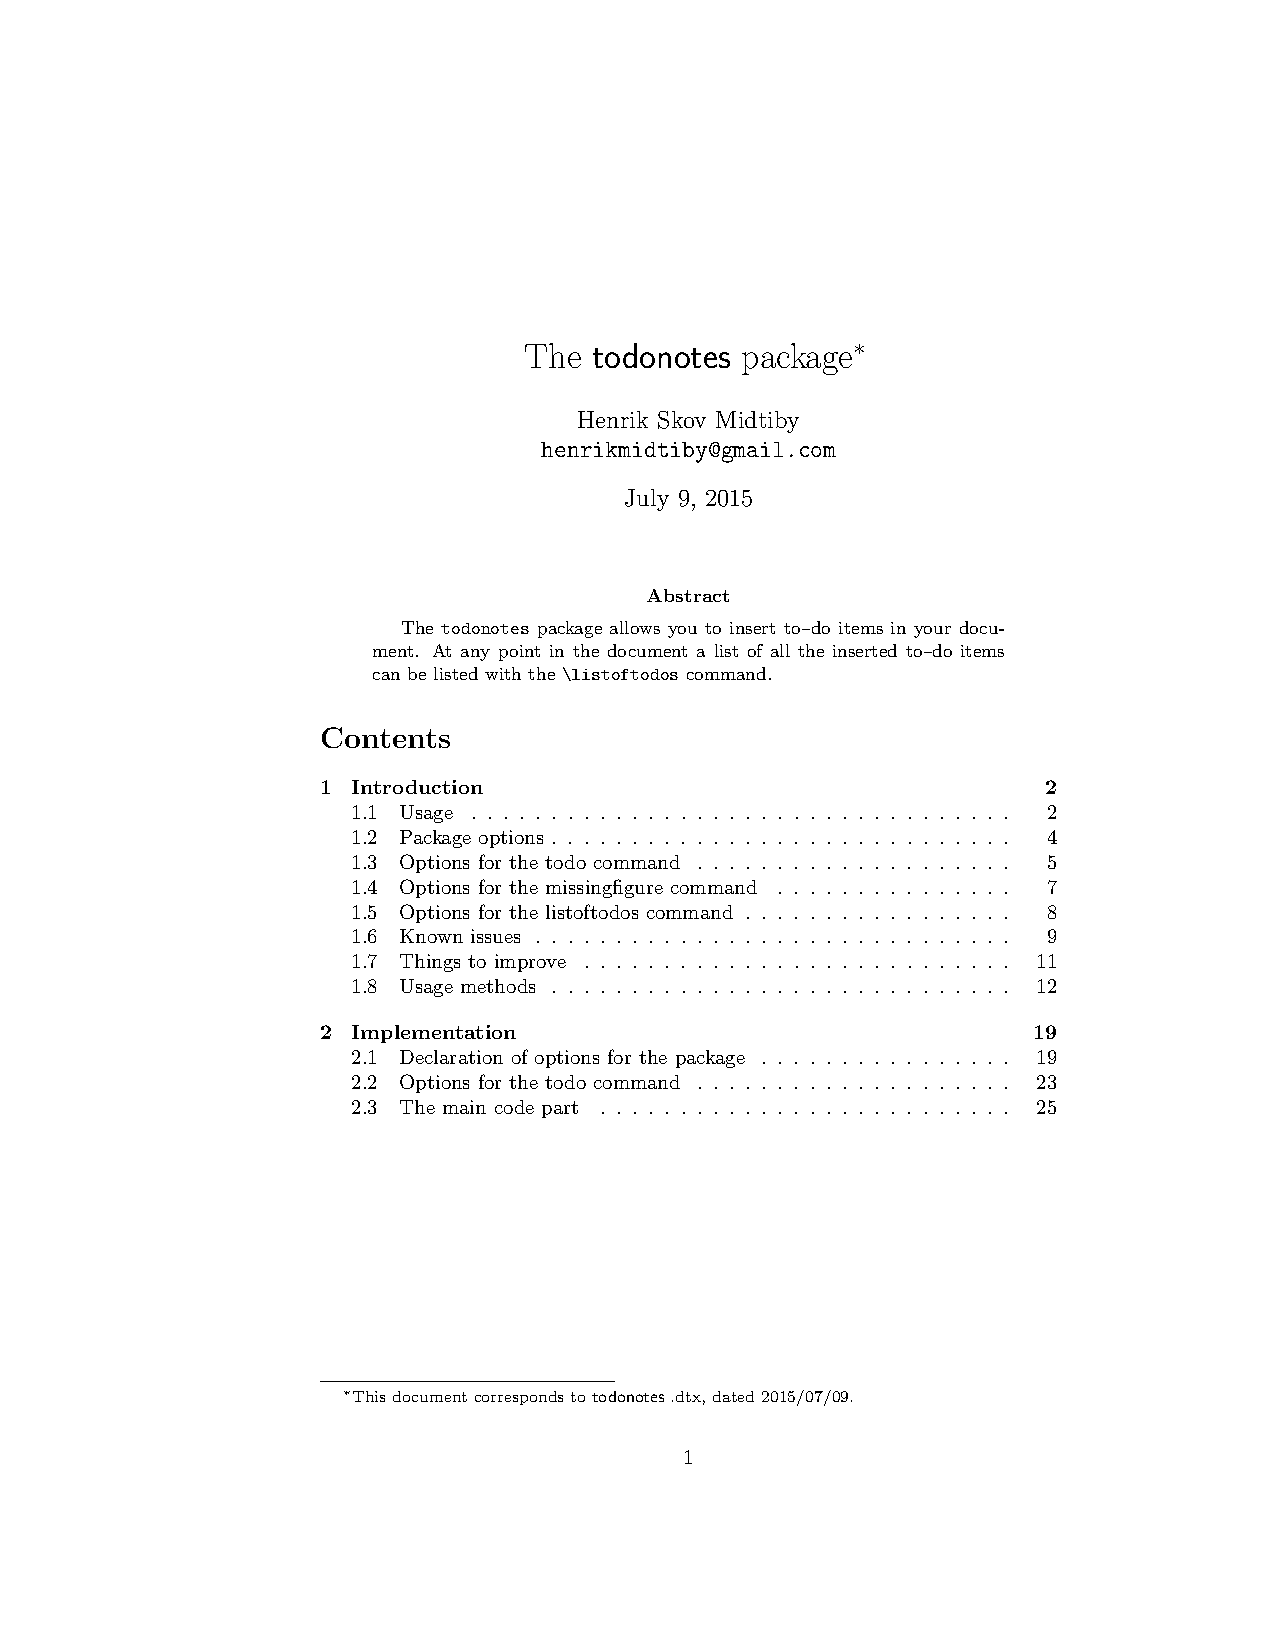
\includepdf[pages=1-3,scale=0.8,frame=true,pagecommand={}]{anexos/todonotes.pdf}


% ---
% Para incluir sem gerar a quebra de página inicial no anexo
\chapter{Publicações no Blog}

Esse apêndice trás os posts do blog semanal para demonstrar o desenvolvimento do projeto ao decorrer da matéria. 

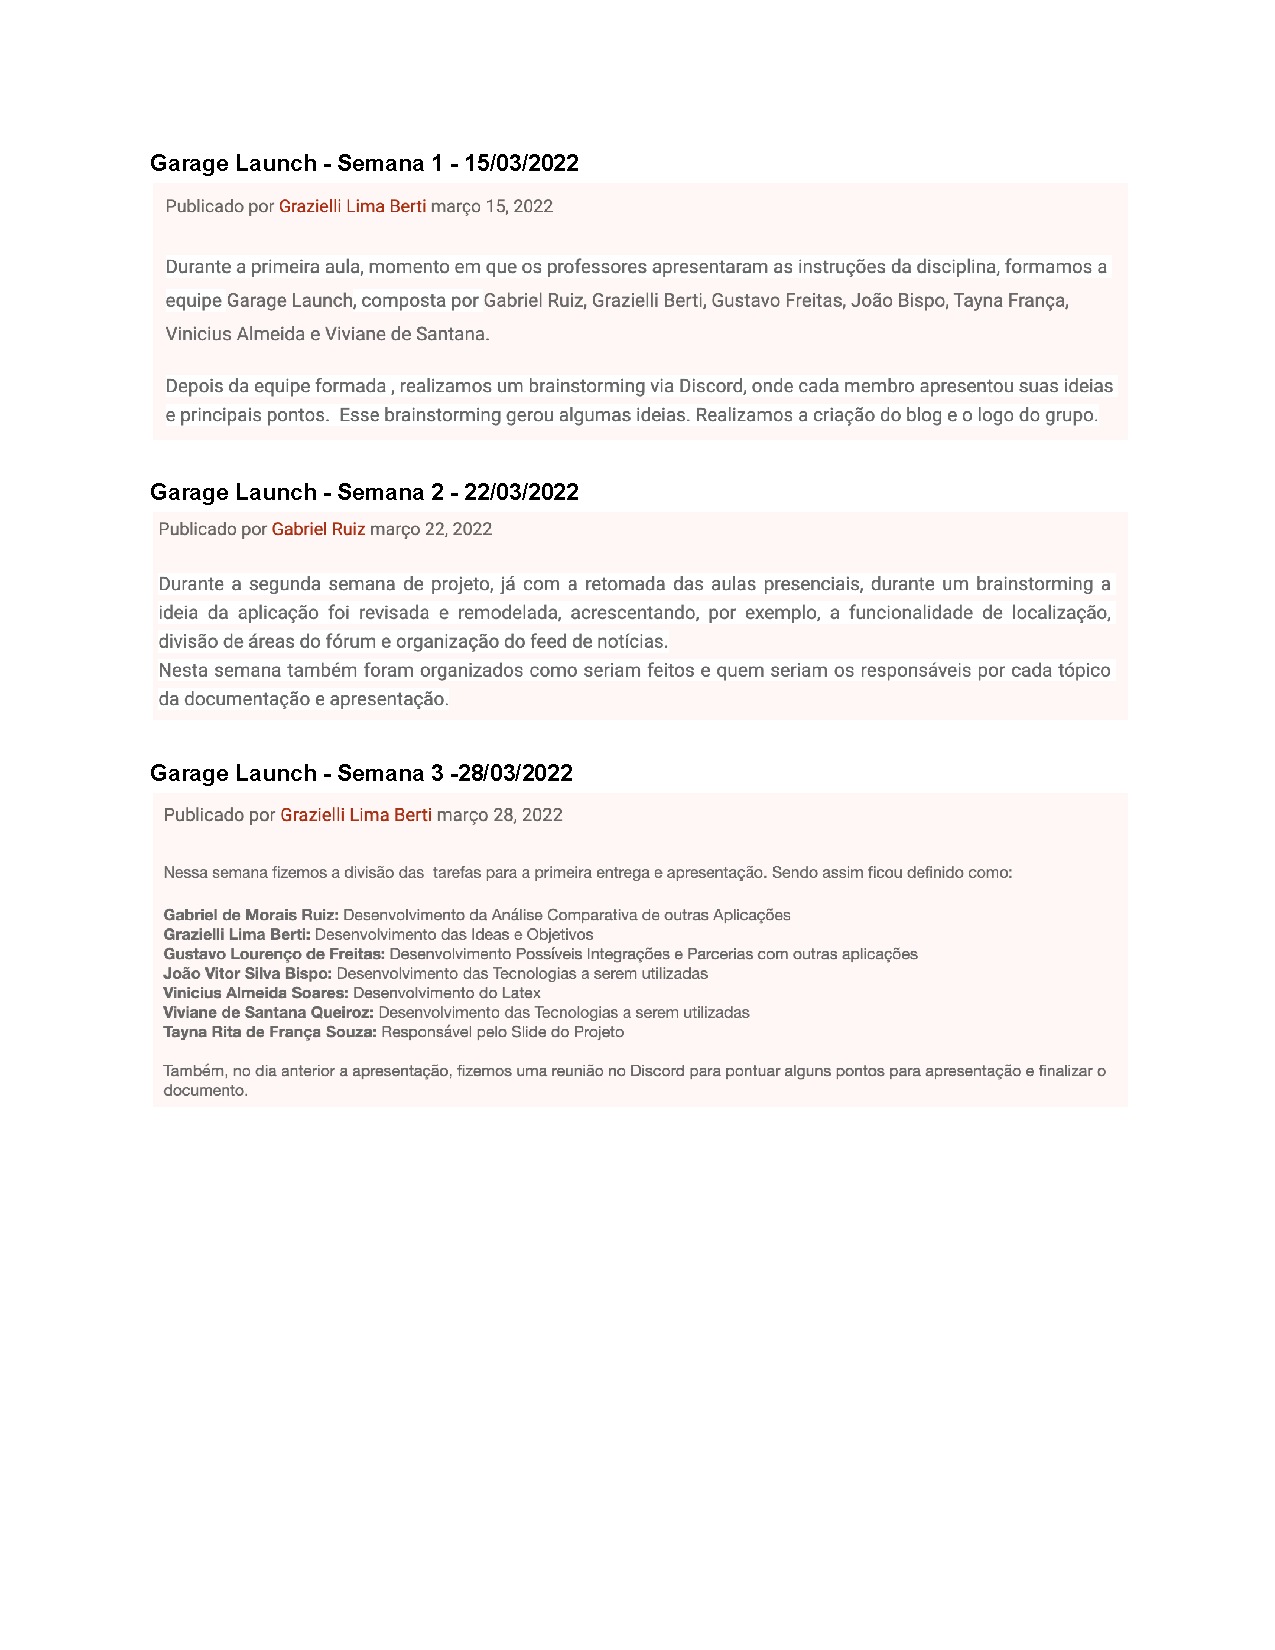
\includepdf[pages=1-6,scale=0.8,frame=true,pagecommand={}\label{publicacao-blog}]{anexos/Anexos_Todos_Os_Post_Do_Blog.pdf}


\end{apendicesenv}
% ---

% ----------------------------------------------------------
% Anexos
% Documentos gerados por outros autores
% ----------------------------------------------------------

% ---
% Inicia os anexos
% ---
\begin{anexosenv}
\anexos
% Imprime uma página indicando o início dos anexos
\partanexos

% ---
\chapter{Manual todonotes(parcial)}
\label{manual-todonotes}
% ---
\index{pdf}
% se pages = "-"  fica com arquivo completo
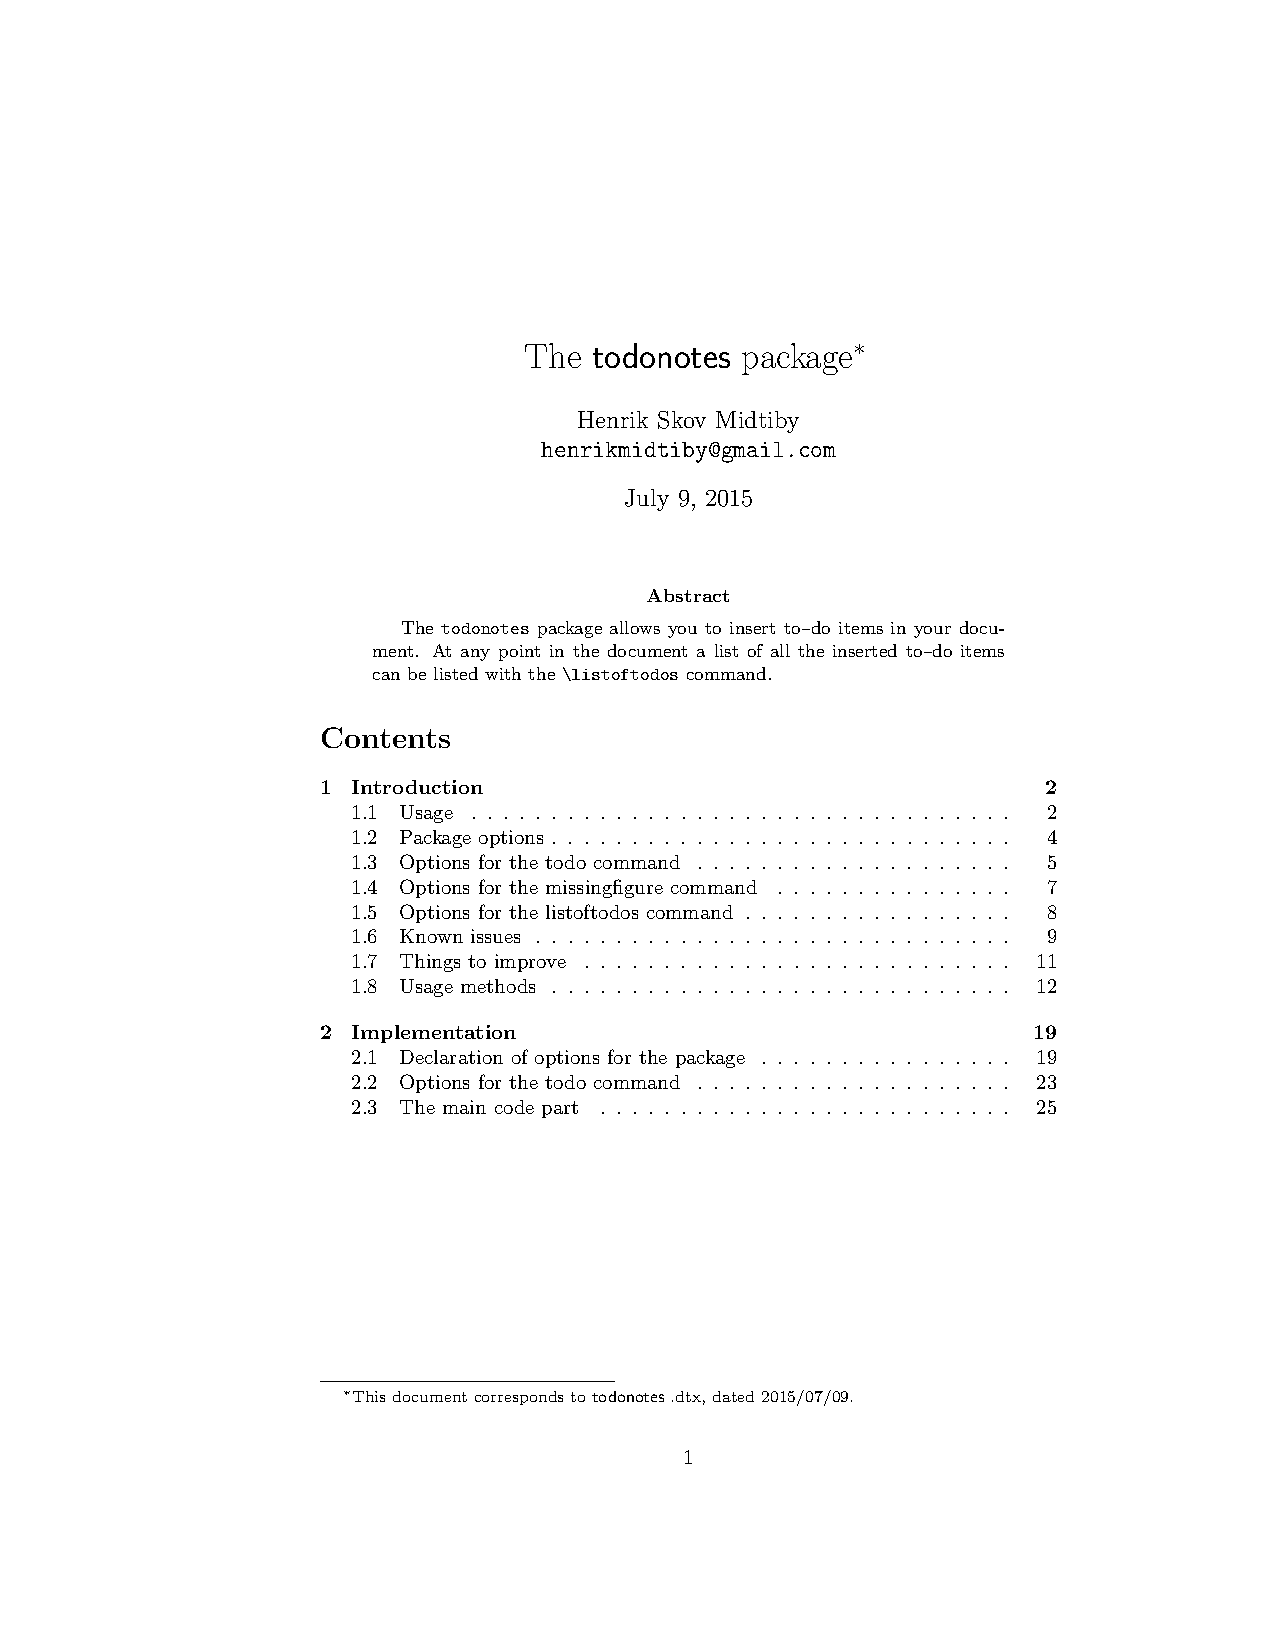
\includepdf[pages=1-3,scale=0.8,frame=true,pagecommand={}]{anexos/todonotes.pdf}

% ---
% Para incluir sem gerar a quebra de página inicial no anexo
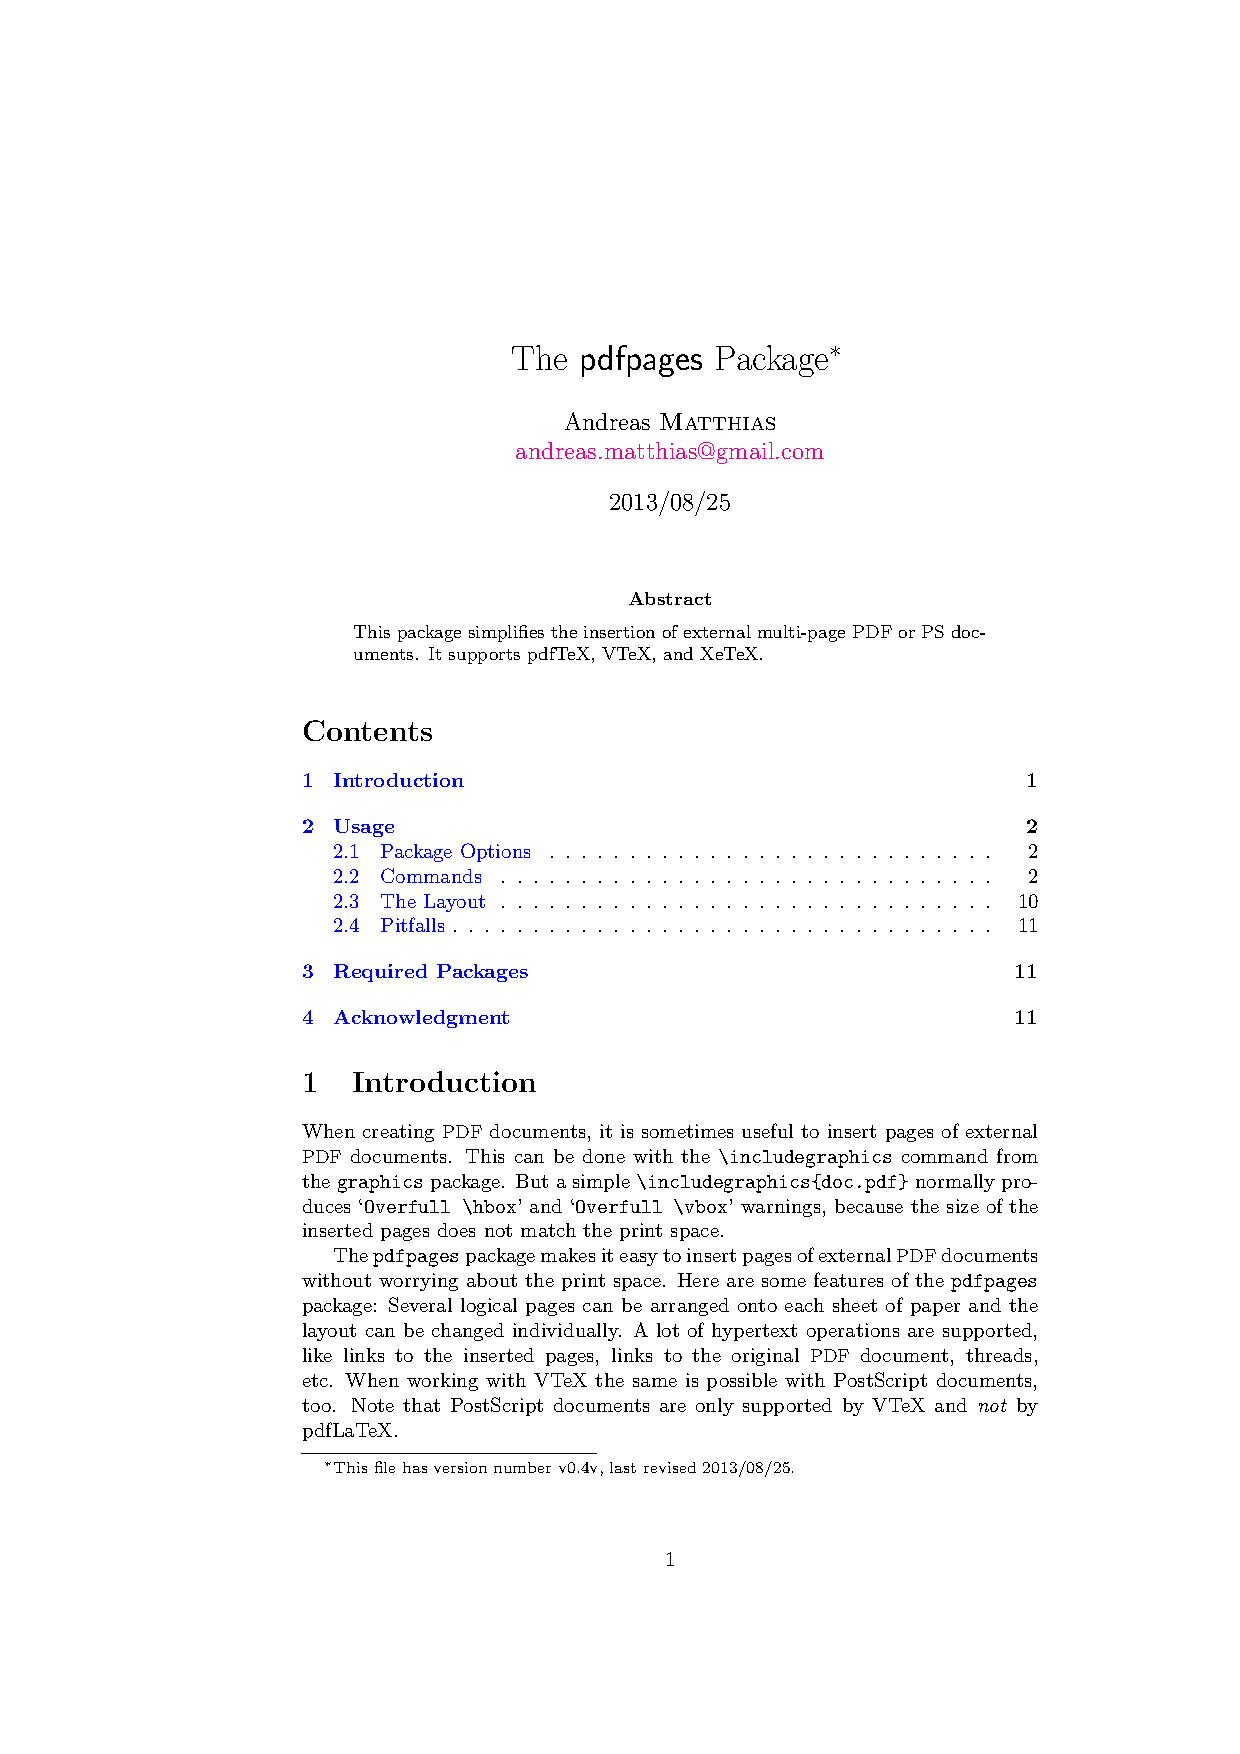
\includepdf[pages=1,scale=0.7,frame=true,pagecommand=\chapter{Manual pdfpages(parcial)}\label{manual-pdfpages}]{anexos/pdfpages.pdf}
\includepdf[pages=2-3,scale=0.8,frame=true,pagecommand={}]{anexos/pdfpages.pdf}

% ---
\chapter{Manual acronym(parcial)}
\index{pdf}
% somente algumas páginas para exemplo sem borda
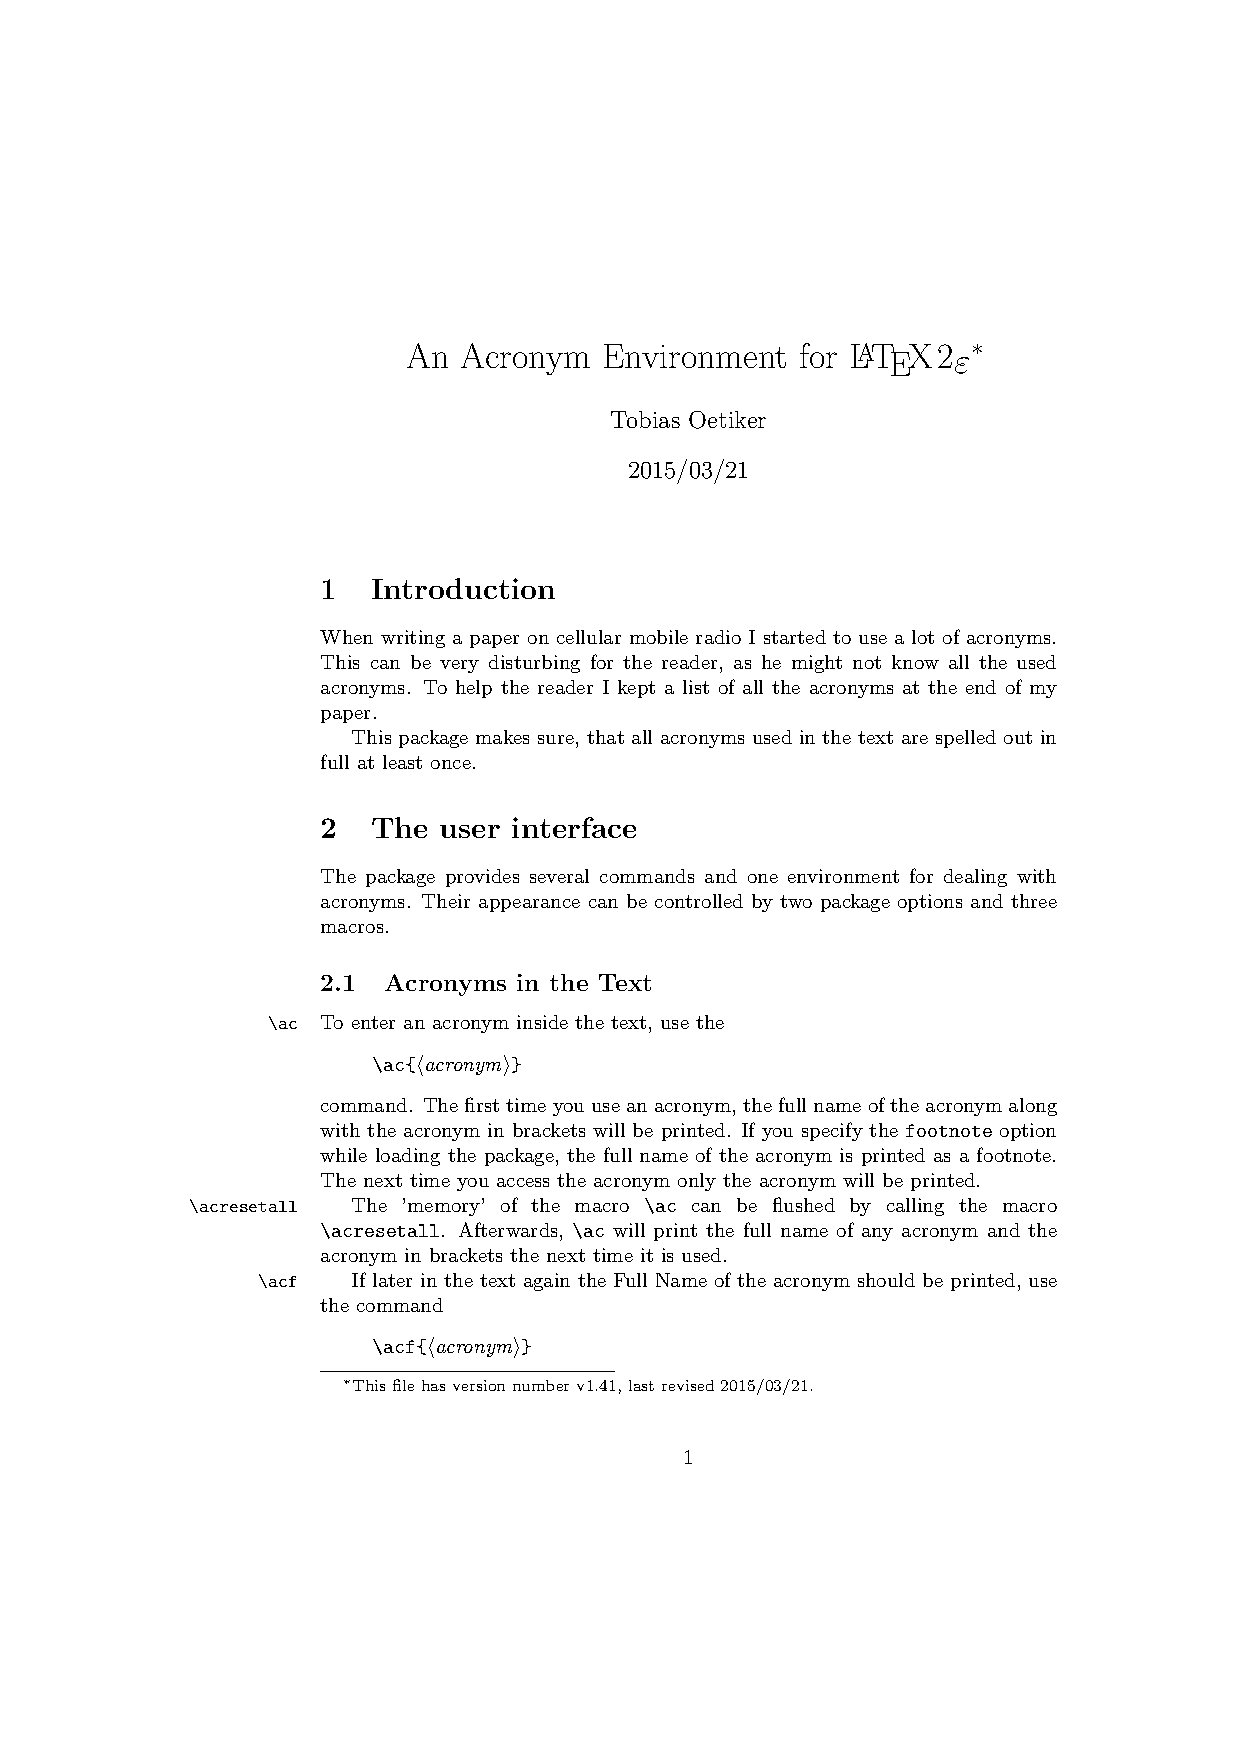
\includepdf[pages=1-3,frame=false,pagecommand={}]{anexos/acronym.pdf}



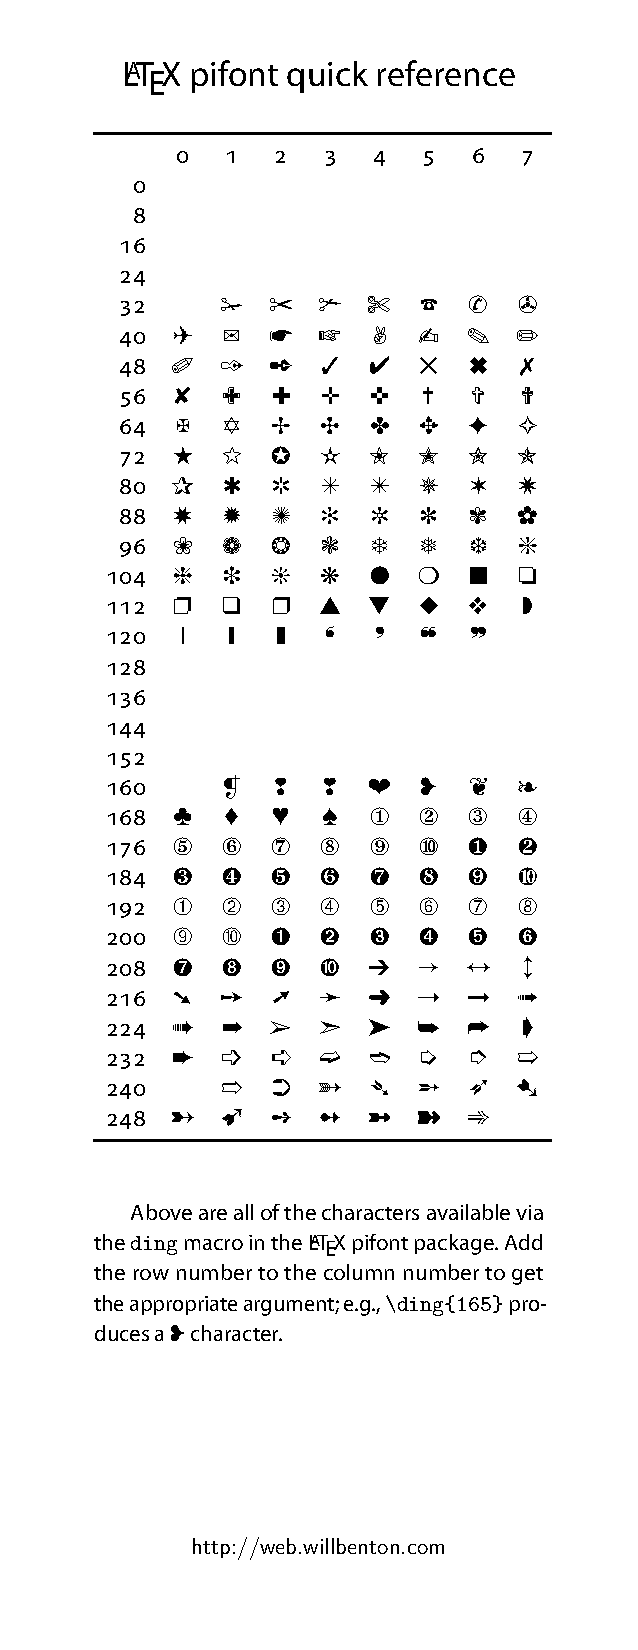
\includepdf[frame=true,scale=0.7,pagecommand=\chapter{Referência Rápida pifont}\label{pifont-quickref}]{anexos/pifont.pdf}


\end{anexosenv}



%---------------------------------------------------------------------
% INDICE REMISSIVO - Quando necessário 
% As palavras indexadas devem ser definidas com \index{} no texto
%---------------------------------------------------------------------
\phantompart
\printindex
\todonum[inline]{remover indice remissivo se não for necessário}

%---------------------------------------------------------------------

\end{document}